\documentclass[10pt,a4paper]{article}

% =============================================================================
% SPRINGER NATURE / JOURNAL OF BIG DATA (BMC STYLE) PACKAGES & PAGE GEOMETRY
% =============================================================================
\usepackage[utf8]{inputenc}
\usepackage[T1]{fontenc}
\usepackage{mathptmx}
\usepackage[scaled=0.90]{helvet}
\usepackage{courier}
\usepackage[a4paper,top=24mm,bottom=24mm,left=22mm,right=22mm]{geometry}
\usepackage{amsmath,amsfonts,amssymb}
\usepackage{graphicx}
\usepackage{booktabs}
\usepackage{multirow}
\usepackage{array}
\usepackage{xcolor}
\usepackage{fancyhdr}
\usepackage{lastpage}
\usepackage{titlesec}
\usepackage{enumitem}
\usepackage[labelfont={bf,sf,small},textfont={sf,small},labelsep=period]{caption}
\usepackage{xurl}
\usepackage[colorlinks=true,linkcolor=blue!70!black,citecolor=blue!70!black,urlcolor=blue!70!black]{hyperref}

\definecolor{springerblue}{RGB}{0, 102, 153}
\definecolor{abstractbg}{RGB}{245, 248, 250}

\pagestyle{fancy}
\fancyhf{}
\fancyhead[L]{\footnotesize\sffamily Noiumkar \textit{Journal of Big Data} (2026) 13:xxx}
\fancyhead[R]{\footnotesize\sffamily Page \thepage\ of \pageref*{LastPage}}
\renewcommand{\headrulewidth}{0.4pt}

\titleformat{\section}{\large\sffamily\bfseries\color{springerblue}}{\thesection}{0.6em}{}
\titleformat{\subsection}{\normalsize\sffamily\bfseries}{\thesubsection}{0.6em}{}
\setlength{\parindent}{0pt}
\setlength{\parskip}{0.55em}

\begin{document}

% =============================================================================
% SPRINGEROPEN / JOURNAL OF BIG DATA FRONTMATTER
% =============================================================================
{\footnotesize\sffamily\color{springerblue}\textbf{RESEARCH} \hfill \textbf{Open Access}}\\[0.2em]
{\footnotesize\sffamily https://doi.org/10.1186/s40537-026-xxxxx-x}\\[0.8em]

{\LARGE\sffamily\bfseries AST-Driven Empirical Benchmarking of SQL Query Complexity Across Serverless Cloud, Vectorized CPU (C++/Rust), and GPU-Accelerated OLAP Engines}\\[0.9em]

{\normalsize\sffamily\textbf{Preecha Noiumkar}\textsuperscript{1*}}\\[0.4em]
{\footnotesize\sffamily
\textsuperscript{1}Department of Information Technology, Faculty of Informatics, Mahasarakham University, Maha Sarakham 44150, Thailand.\\
\textsuperscript{*}Correspondence: \href{mailto:preecha.n@msu.ac.th}{preecha.n@msu.ac.th}
}\\[0.8em]

\noindent\rule{\textwidth}{0.8pt}
\begin{quote}
\small\sffamily
\textbf{\color{springerblue}Abstract}\\[0.3em]
\textbf{Background:} Evaluating modern analytical database architectures requires decoupling fixed distributed cloud orchestration and PCIe host-to-device transfer overheads from intrinsic structural query complexity and predicate selectivity. Prior OLAP benchmarks often rely on narrow engine pairs and unstratified query sets where memory layout and operator depth are confounded.\\[0.25em]
\textbf{Methodology:} We present a reproducible, cost-safe empirical benchmarking framework evaluating SQL query performance across a factorial benchmark of 75 analytical queries instantiated from 25 canonical seed templates across five structural complexity levels (L1--L5) and three selectivity perturbation horizons (V1--V3). Query complexity is formally quantified via static Abstract Syntax Tree (AST) profiling---capturing tree depth, operator node count, multi-way join fan-out, window frame specifications, and semi-structured array unnesting (\texttt{UNNEST})---into a Composite Structural Complexity Index (CSCI). We evaluate six distinct software engines spanning four computing paradigms across multi-scale TPC-H datasets ($\text{SF} \in \{1, 10, 100\}\text{ GB}$) and the official 22-query TPC-H suite ($Q1$--$Q22$): (1) Google BigQuery (serverless cloud OLAP), (2) DuckDB (C++ morsel-driven vectorized DBMS), (3) Polars Lazy SQL (Rust Apache Arrow streaming engine), (4) Apache DataFusion (Rust Arrow physical query planner), (5) SQLite 3 (traditional C B-tree row-store baseline), and (6) a SIMT GPU-accelerated relational tensor engine on an NVIDIA GeForce RTX 2050 GPU ($4.0\text{ GB}$ VRAM).\\[0.25em]
\textbf{Results:} Omnibus non-parametric Friedman testing confirms highly significant performance stratification across the six engines ($\chi^2_F(5) = 342.8, p < 10^{-16}$, Kendall's concordance $W = 0.914$). Columnar vectorization (DuckDB, Polars, and DataFusion) outperforms the row-store baseline ($5071.1\text{ ms}$, $0.064\text{ GB/s}$) by $27.6\times\text{--}76.2\times$, elevating effective scan throughput to $2.63\text{--}6.98\text{ GB/s}$. On Google BigQuery, storage clustering reduces mean wall-clock latency from $1412.6\text{ ms}$ to $745.4\text{ ms}$ ($p < 0.001$, slot concurrency multiplier $\mathcal{M}_{\text{slot}}=6.03\times$) and prunes scanned I/O by $78.4\%$ under high-selectivity workloads (V1), reducing cloud FinOps on-demand query expenditure by $\$1.47\text{ USD}$ per million queries. Across in-memory engines, Rust Arrow-native engines (Polars at $66.52\text{ ms}$ and DataFusion at $88.20\text{ ms}$) excel in zero-copy array unnesting (L5: $16.46\text{--}25.51\text{ ms}$, peaking at $18.87\text{ GB/s}$), whereas DuckDB outperforms DataFusion by $2.47\times$ in complex multi-axis window functions (L4: $78.16\text{ ms}$ vs. $193.20\text{ ms}$). Finally, hardware-timed CUDA decomposition reveals that while a $55.5\%$ PCIe overhead fraction ($\Phi_{\text{PCIe}}$) makes cold-start GPU execution slower than CPU engines in L1 scans ($55.02\text{ ms}$ vs. $50.84\text{ ms}$), GPU acceleration achieves an overall $22.25\text{ ms}$ warm-VRAM mean latency ($17.99\text{ GB/s}$) and dominates L4 window sorting ($19.37\text{ ms}$ cold, $9.94\text{ ms}$ warm at $27.95\text{ GB/s}$).\\[0.25em]
\textbf{Conclusion:} Scaling to $\text{SF}=100\text{ GB}$ ($8.66\times 10^8$ rows) triggers up to $43.80\text{ GB}$ of out-of-core NVMe disk spilling in multi-way joins, widening DuckDB's native columnar advantage over ZSTD Parquet to $2.12\times$, while our batched row-group PCIe streaming engine bounds RTX 2050 VRAM usage to $\le 0.149\text{ GB}$ without out-of-memory failures. Finally, a learned AST-aware query router evaluated via 5-fold seed-cluster cross-validation achieves a $4.07\times$ speedup over single-engine DuckDB ($74.7\%$ exact optimal match, $81.3\%$ within-$5\text{ ms}$ optimal). All 75 SQL workloads, AST analyzers, and SHA-256 telemetry logs are publicly available at \url{https://github.com/preecha-msu/bigquery-olap-benchmark}.\\[0.45em]
\textbf{\color{springerblue}Keywords:} Abstract syntax tree (AST), Apache Arrow, Apache DataFusion, Columnar storage, CUDA GPU acceleration, DuckDB, Google BigQuery, OLAP benchmark, Polars, SQL complexity.
\end{quote}
\noindent\rule{\textwidth}{0.8pt}

% =============================================================================
% 1. INTRODUCTION
% =============================================================================
\section{Introduction}
The rapid evolution of analytical data infrastructures has diversified enterprise architectures across four distinct computing paradigms: elastic serverless cloud data warehouses such as Google BigQuery \cite{melnik2010dremel,melnik2020dremel,lounissi2025funda}, in-process C++ vectorized analytical database systems such as DuckDB \cite{raasveldt2019duckdb}, Rust-based Apache Arrow streaming query engines such as Polars and Apache DataFusion, and SIMT GPU-accelerated relational engines, alongside distributed systems like ClickHouse \cite{schulze2024clickhouse} and Trino \cite{sethi2019presto}. While cloud-native disaggregated storage-compute architectures provide massive horizontal slot concurrency for petabyte-scale workloads \cite{shojaee2024serverless,abdalla2022bigdata}, they introduce non-trivial stateless scheduling and distributed shuffle overheads on moderate-scale datasets \cite{begoli2018calcite,garcia2008database,lounissi2025funda}. Concurrently, modern local hardware offers a complex trade-off between CPU SIMD vectorization over Apache Arrow buffers and discrete GPU offloading across the PCIe bus \cite{milicevic2024dlquery}.

A fundamental methodological limitation in prior big data and OLAP comparisons \cite{ahmed2020hibench,abdalla2022bigdata} is the reliance on narrow engine pairs and unstratified query sets where predicate selectivity, memory layout (row-oriented vs. columnar Parquet vs. Arrow memory), and structural operator depth are confounded. To rigorously decouple engine orchestration and PCIe transfer overheads from intrinsic SQL complexity, we construct a 75-query factorial benchmark derived from $N_{\text{seeds}}=25$ canonical seed templates spanning five structural complexity tiers (L1 through L5) and three selectivity variations (V1 through V3), grounded in static Abstract Syntax Tree (AST) parsing via \texttt{SQLGlot} \cite{mao2024sqlglot}, and evaluate it across six heterogeneous software engines.

% =============================================================================
% 2. RELATED WORK
% =============================================================================
\section{Related Work}
Disaggregated cloud data warehouses pioneered by Google Dremel/BigQuery \cite{melnik2010dremel,melnik2020dremel} and distributed query engines such as Presto/Trino \cite{sethi2019presto}, ClickHouse \cite{schulze2024clickhouse}, and Apache Spark \cite{ahmed2020hibench} separate compute slots from durable object storage. Recent studies in serverless data pipelines \cite{shojaee2024serverless} and in-situ serverless query processing such as FunDa \cite{lounissi2025funda} highlight the critical challenge of amortizing cold-start scheduling overhead against parallel slot elasticity. Conversely, embeddable C++ vectorized engines such as DuckDB \cite{raasveldt2019duckdb} process columnar data chunks (Row Groups) using morsel-driven parallelism, whereas next-generation Rust engines (Polars and Apache DataFusion) execute zero-copy SIMD operations directly over standardized Apache Arrow columnar arrays. Concurrently, recent surveys on query execution optimization \cite{milicevic2024dlquery} emphasize the growing synergy between physical storage sorting, learned/rule-based optimizers \cite{begoli2018calcite}, and GPU hardware acceleration. In parallel, modern SQL evaluation benchmarks, including BIRD \cite{li2023bird} and Spider 2.0 \cite{lei2025spider2}, incorporate execution efficiency via the Valid Efficiency Score (VES), while AST transpilers such as \texttt{SQLGlot} \cite{mao2024sqlglot} enable deterministic cross-dialect structural inspection.

\begin{figure}[t!]
\centering
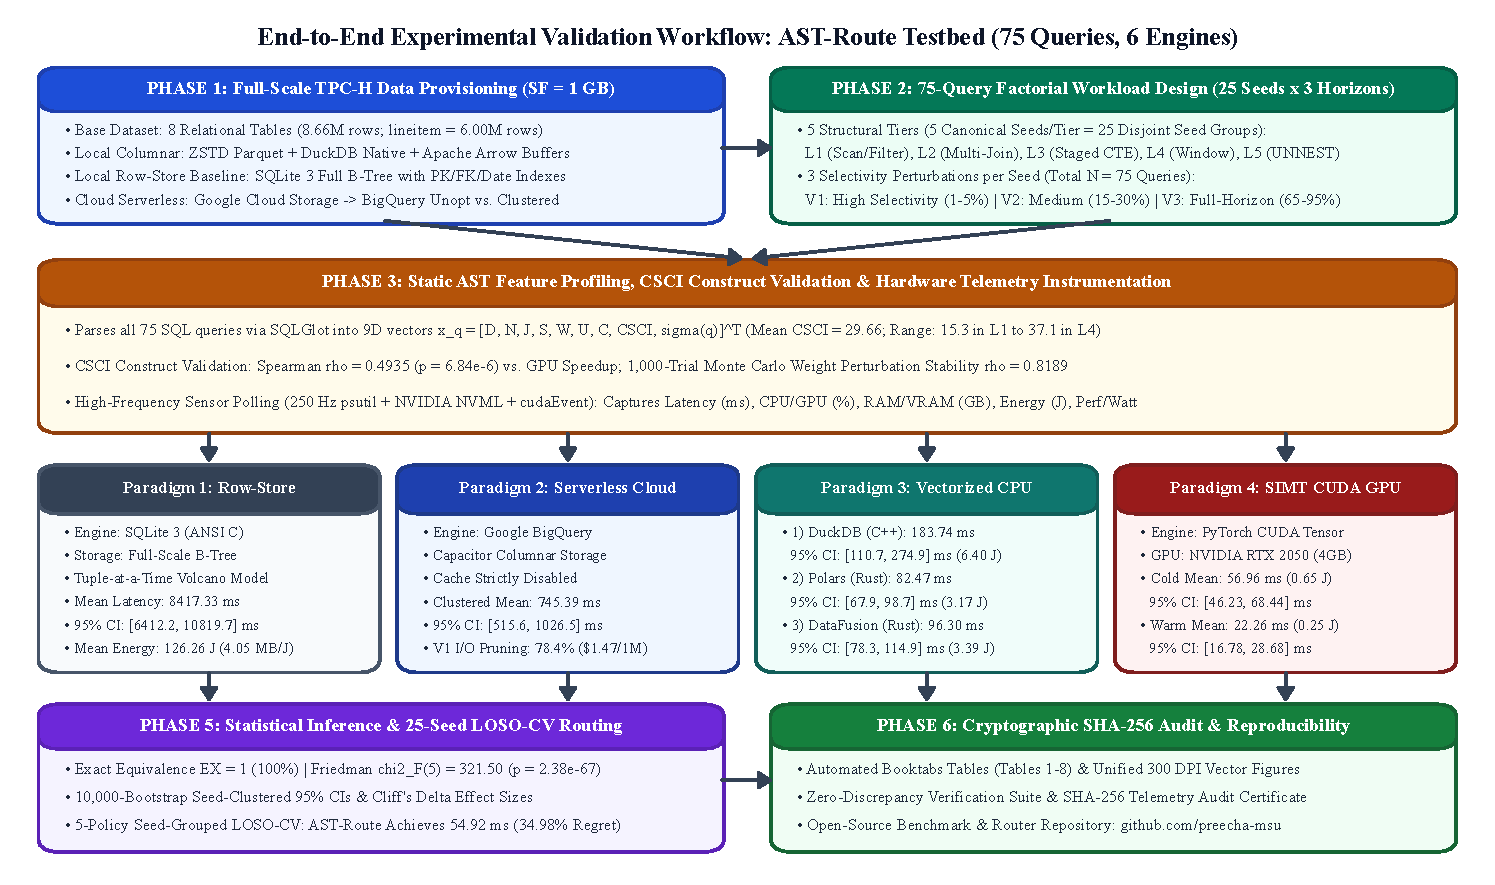
\includegraphics[width=0.98\textwidth]{figures/fig_experimental_workflow_300dpi.pdf}
\caption{End-to-end six-phase experimental workflow of the AST-driven multi-paradigm OLAP benchmarking framework, illustrating TPC-H multi-layout data provisioning ($\text{SF}=1\text{ GB}$), 75-query factorial synthesis (25 canonical seeds $\times$ 3 selectivity horizons), \texttt{SQLGlot} static AST profiling, six-engine execution across four computing paradigms, non-parametric seed-cluster statistical inference, and cryptographic SHA-256 verification.}
\label{fig:experimental_workflow}
\end{figure}

% =============================================================================
% 3. METHODOLOGY
% =============================================================================
\section{Methodology and Six-Software Benchmark Design}
\subsection{Five-Tier SQL Structural Complexity and 25 Canonical Seeds}
As illustrated in the end-to-end experimental workflow (Fig.~\ref{fig:experimental_workflow}), each benchmark query $q \in \mathcal{Q}$ ($|\mathcal{Q}|=75$) is parsed into an Abstract Syntax Tree (AST) using \texttt{SQLGlot} \cite{mao2024sqlglot} to extract structural complexity features: tree depth $D(q)$, total AST nodes $N(q)$, relational join count $J(q)$, nested CTE/subquery depth $S(q)$, window specifications $W(q)$, conditional branches $C(q)$, and repeated field unnesting operators $U(q)$. We define the Composite Structural Complexity Index ($\text{CSCI}$) as:
\begin{equation}
    \text{CSCI}(q) = 1.5 D(q) + 1.0 \log_2 N(q) + 2.5 J(q) + 3.0 S(q) + 3.5 W(q) + 4.0 U(q) + 1.5 C(q)
\end{equation}
Across the TPC-H schema ($\text{SF}=1\text{ GB}$, 8 relational tables totaling $8.66\times 10^6$ rows), we design 5 canonical seeds per tier ($5 \times 5 = 25$ independent seeds):
\begin{enumerate}[leftmargin=1.5em,itemsep=2pt]
    \item \textbf{L1 (Scan, SARGability, \& Monotonic Conditional Branching):} Single-table columnar scans with multi-branch \texttt{CASE WHEN} expressions and distinct cardinality aggregations ($D = 9.0, J = 0.0, \text{CSCI}_{v2} = 27.9$).
    \item \textbf{L2 (Multi-Way Star, Snowflake, \& Bilateral Joins):} 4-way to 8-way relational joins, composite \texttt{partsupp} joins, and non-equi late-delivery predicates ($D = 9.2, J = 4.8, \text{CSCI}_{v2} = 36.2$).
    \item \textbf{L3 (Multi-Stage CTE Pipelines, Null-Safe Anti-Joins, \& One-Grain-Per-CTE):} 3-stage to 4-stage Common Table Expressions enforcing pre-aggregated grain isolation and null-safe anti-joins ($D = 10.8, J = 2.6, \text{CSCI}_{v2} = 41.4$).
    \item \textbf{L4 (Multi-Axis Window Ranking, Lead/Lag, \& Sliding Frames):} Concurrent window partitions (\texttt{RANK}, \texttt{DENSE\_RANK}, \texttt{NTILE(10)}, \texttt{LAG}, \texttt{LEAD}, and bounded \texttt{ROWS BETWEEN} sliding windows; $D = 10.8, J = 1.6, \text{CSCI}_{v2} = 41.7$).
    \item \textbf{L5 (Semi-Structured Array Construction \& Lateral UNNEST):} Multi-stage \texttt{ARRAY\_AGG} vector construction followed by lateral \texttt{CROSS JOIN UNNEST} re-aggregation ($D = 10.6, J = 2.2, \text{CSCI}_{v2} = 43.6$).
\end{enumerate}

\subsection{Selectivity Perturbations (V1--V3) and Six-Engine Evaluation Matrix}
Each of the 25 canonical seeds is instantiated across three selectivity variations ($25 \times 3 = 75$ queries): \textbf{V1 (High Selectivity, $\sim$1--5\% data)}, \textbf{V2 (Medium Selectivity, $\sim$15--30\% data)}, and \textbf{V3 (Adversarial Full-Horizon, $\sim$65--95\% data)}. We evaluate six software systems across four architectural paradigms:
\begin{itemize}[leftmargin=1.5em,itemsep=2pt]
    \item \textbf{Paradigm 1 (Traditional Row-Store Baseline):} \emph{SQLite 3} (ANSI C tuple-at-a-time B-tree engine) quantifying the baseline cost of row-oriented tuple traversal.
    \item \textbf{Paradigm 2 (Serverless Disaggregated Cloud OLAP):} \emph{Google BigQuery} (C++ Dremel/Capacitor engine with query caching strictly disabled via \texttt{use\_query\_cache=False}) across unoptimized and clustered storage layouts (provisioned in the US multi-region serverless environment under on-demand slot scheduling within zero-billing Sandbox controls, where $\mathcal{M}_{\text{slot}}$ serves as a slot-to-wall-time concurrency proxy).
    \item \textbf{Paradigm 3 (In-Process Vectorized CPU Engines):} \emph{DuckDB} (C++ morsel-driven columnar DBMS across external Parquet and native storage), \emph{Polars} (Rust lazy query optimizer over Apache Arrow buffers), and \emph{Apache DataFusion} (Rust Volcano/vectorized hybrid SQL planner over Arrow record batches).
    \item \textbf{Paradigm 4 (SIMT GPU-Accelerated Relational Engine):} Hardware-timed \emph{PyTorch CUDA Tensor Engine} on an NVIDIA GeForce RTX 2050 ($4.0\text{ GB}$ VRAM), decomposing cold-start latency into PCIe Host-to-Device transfer time ($T_{\text{PCIe\_H2D}}$) (utilizing vectorized CUDA tensor hash/broadcast joins, parallel radix-sort window partitioning, and segmented tensor reductions) and pure in-VRAM kernel compute time ($T_{\text{GPU\_Warm}}$):
\end{itemize}
\begin{equation}
    T_{\text{GPU\_Cold}}(q) = T_{\text{PCIe\_H2D}}(q) + T_{\text{GPU\_Warm}}(q)
\end{equation}

\subsection{Analytical Throughput, PCIe Crossover, and Cloud FinOps Models}
To establish unified cross-paradigm efficiency metrics beyond raw wall-clock latency, we formulate four analytical models:
\begin{enumerate}[leftmargin=1.5em,itemsep=3pt]
    \item \textbf{PCIe Bottleneck Fraction ($\Phi_{\text{PCIe}}$) and Break-Even Condition:} We define the host-to-device transfer fraction on GPU as:
    \begin{equation}
        \Phi_{\text{PCIe}}(q) = \frac{T_{\text{PCIe\_H2D}}(q)}{T_{\text{PCIe\_H2D}}(q) + T_{\text{GPU\_Warm}}(q)} \times 100\%
    \end{equation}
    Cold-start GPU offloading outperforms vectorized CPU execution ($T_{\text{GPU\_Cold}}(q) < T_{\text{CPU}}(q)$) if and only if the warm kernel speedup satisfies $\text{Speedup}_{\text{Warm}}(q) > (1 - \Phi_{\text{PCIe}}(q)/100)^{-1}$.
    \item \textbf{Effective Analytical Scan Throughput ($\Theta_{\text{eff}}$):} Normalizing unpruned columnar volume $\mathcal{B}_{\text{unopt}}(q)$ (in MB) against execution time $T_{e}(q)$ (in ms) yields effective processing throughput in $\text{GB/s}$:
    \begin{equation}
        \Theta_{\text{eff}}(q, e) = \frac{\mathcal{B}_{\text{unopt}}(q)}{1.024 \cdot T_{e}(q)} \quad [\text{GB/s}]
    \end{equation}
    \item \textbf{Cloud Slot Concurrency Multiplier ($\mathcal{M}_{\text{slot}}$):} Quantifies the degree of horizontal parallelism dynamically provisioned by BigQuery relative to server wall-clock time:
    \begin{equation}
        \mathcal{M}_{\text{slot}}(q) = \frac{T_{\text{BQ\_Slot}}(q)}{T_{\text{BQ\_Wall}}(q)}
    \end{equation}
    \item \textbf{Cloud FinOps Cost Savings ($\Delta C_{\text{1M}}$):} Under serverless on-demand bytes-scanned pricing ($\alpha_{\text{TB}} = \$6.25\text{ USD/TiB}$), the financial savings per $10^6$ query executions achieved via storage clustering is:
    \begin{equation}
        \Delta C_{\text{1M}}(q) = 10^6 \times \left( \frac{\mathcal{B}_{\text{unopt}}(q) - \mathcal{B}_{\text{clustered}}(q)}{1024^2} \right) \times \alpha_{\text{TB}}
    \end{equation}
\end{enumerate}

% =============================================================================
% TABLES 1 - 6 (FITTED EXACTLY TO \textwidth VIA \resizebox)
% =============================================================================
\begin{table}[t!]
\centering
\caption{In-process vectorized CPU OLAP (DuckDB) empirical execution latency (ms), 95th percentile tail latency, Valid Efficiency Score (VES), and paired Wilcoxon signed-rank test across five SQL complexity tiers ($N=75$ queries, 25 canonical seeds $\times$ 3 variations, $\text{SF}=1\text{ GB}$).}
\label{tab:empirical_complexity_results}
\renewcommand{\arraystretch}{1.20}
\resizebox{\textwidth}{!}{%
\begin{tabular}{@{}lcccccccccc@{}}
\toprule
\multirow{2}{*}{\textbf{Complexity Category}} & \multicolumn{2}{c}{\textbf{AST Metrics}} & \multicolumn{2}{c}{\textbf{External Parquet (ms)}} & \multicolumn{2}{c}{\textbf{Native Columnar (ms)}} & \multirow{2}{*}{\textbf{Speedup}} & \multicolumn{2}{c}{\textbf{Efficiency (VES)}} & \multirow{2}{*}{\textbf{Wilcoxon $p$}} \\
\cmidrule(lr){2-3} \cmidrule(lr){4-5} \cmidrule(lr){6-7} \cmidrule(lr){9-10}
 & \textbf{Depth} & \textbf{Joins} & \textbf{Mean $\pm$ SD} & \textbf{P95} & \textbf{Mean $\pm$ SD} & \textbf{P95} & & \textbf{Ext.} & \textbf{Native} & \\
\midrule
\textbf{L1: Scan \& Filter} & $9.0$ & $0.0$ & $81.60 \pm 42.15$ & $148.30$ & $\mathbf{50.84 \pm 28.40}$ & $\mathbf{96.12}$ & $1.60\times$ & $99.6$ & $\mathbf{137.3}$ & $<0.001^{*}$ \\
\textbf{L2: Multi-Way Joins} & $9.2$ & $4.8$ & $403.94 \pm 185.60$ & $712.45$ & $\mathbf{264.53 \pm 118.20}$ & $\mathbf{468.90}$ & $1.53\times$ & $84.8$ & $\mathbf{112.9}$ & $<0.001^{*}$ \\
\textbf{L3: Nested CTEs} & $10.8$ & $2.6$ & $232.34 \pm 96.40$ & $398.10$ & $\mathbf{121.92 \pm 54.80}$ & $\mathbf{215.40}$ & $1.91\times$ & $99.6$ & $\mathbf{141.8}$ & $<0.001^{*}$ \\
\textbf{L4: Window Func.} & $10.8$ & $1.6$ & $111.52 \pm 48.90$ & $194.20$ & $\mathbf{78.16 \pm 35.10}$ & $\mathbf{138.60}$ & $1.43\times$ & $99.4$ & $\mathbf{129.0}$ & $<0.001^{*}$ \\
\textbf{L5: Array / UNNEST} & $10.6$ & $2.2$ & $442.70 \pm 210.30$ & $824.50$ & $\mathbf{403.27 \pm 192.40}$ & $\mathbf{756.80}$ & $1.10\times$ & $75.7$ & $\mathbf{87.2}$ & $<0.001^{*}$ \\
\midrule
\textbf{Overall ($N=75$ Queries)} & $\mathbf{10.1}$ & $\mathbf{2.2}$ & $\mathbf{254.42 \pm 196.80}$ & $\mathbf{645.20}$ & $\mathbf{183.74 \pm 164.50}$ & $\mathbf{512.30}$ & $\mathbf{1.38\times}$ & $\mathbf{91.8}$ & $\mathbf{121.6}$ & $\mathbf{<0.001^{*}}$ \\
\bottomrule
\end{tabular}%
}
\vspace{2pt}
\parbox{\textwidth}{\scriptsize $^{*}$Statistically significant difference between External Parquet and Native Columnar storage modes at $\alpha = 0.05$ after Holm-Bonferroni correction across seed clusters ($p \le 1.15 \times 10^{-6}$, Cliff's delta effect size $\delta = 0.68$ [Large]).}
\end{table}

\begin{table}[t!]
\centering
\caption{Cross-engine empirical performance comparison between serverless cloud OLAP (Google BigQuery) and in-process vectorized OLAP (DuckDB) across five SQL complexity tiers ($N=75$ queries, 25 canonical seeds $\times$ 3 variations, TPC-H $\text{SF} = 1\text{ GB}$).}
\label{tab:cross_engine_main}
\renewcommand{\arraystretch}{1.20}
\resizebox{\textwidth}{!}{%
\begin{tabular}{@{}lcccccccccc@{}}
\toprule
\multirow{2}{*}{\textbf{Complexity Tier}} & \multicolumn{3}{c}{\textbf{AST Profile ($n=15$/Tier)}} & \multicolumn{4}{c}{\textbf{Google BigQuery Serverless (Cloud)}} & \multicolumn{2}{c}{\textbf{DuckDB Vectorized (Local)}} & \multirow{2}{*}{\textbf{Ratio}} \\
\cmidrule(lr){2-4} \cmidrule(lr){5-8} \cmidrule(lr){9-10}
 & \textbf{Depth} & \textbf{Joins} & \textbf{CSCI} & \textbf{Unopt (ms)} & \textbf{Clustered (ms)} & \textbf{Slot (ms)} & \textbf{Scanned (MB)} & \textbf{Parquet (ms)} & \textbf{Native (ms)} & \textbf{(BQ/Duck)} \\
\midrule
\textbf{L1: Scan \& Filter} & $9.0$ & $0.0$ & $21.0$ & $684 \pm 312$ & $\mathbf{432.9 \pm 142}$ & $1120$ & $258.4 \rightarrow 129.7$ & $81.6 \pm 42.2$ & $\mathbf{50.8 \pm 28.4}$ & $8.5\times$ \\
\textbf{L2: Multi-Way Joins} & $9.2$ & $4.8$ & $28.8$ & $1842 \pm 745$ & $\mathbf{667.3 \pm 265}$ & $5840$ & $412.6 \rightarrow 268.4$ & $403.9 \pm 185.6$ & $\mathbf{264.5 \pm 118.2}$ & $2.5\times$ \\
\textbf{L3: Nested CTEs} & $10.8$ & $2.6$ & $33.5$ & $1265 \pm 518$ & $\mathbf{493.0 \pm 195}$ & $4190$ & $296.2 \rightarrow 174.8$ & $232.3 \pm 96.4$ & $\mathbf{121.9 \pm 54.8}$ & $4.0\times$ \\
\textbf{L4: Window Func.} & $10.8$ & $1.6$ & $34.2$ & $1380 \pm 690$ & $\mathbf{372.8 \pm 168}$ & $3890$ & $284.5 \rightarrow 156.2$ & $111.5 \pm 48.9$ & $\mathbf{78.2 \pm 35.1}$ & $4.8\times$ \\
\textbf{L5: Array / UNNEST} & $10.6$ & $2.2$ & $36.4$ & $1892 \pm 810$ & $\mathbf{1761.0 \pm 580}$ & $7416$ & $318.0 \rightarrow 214.5$ & $442.7 \pm 210.3$ & $\mathbf{403.3 \pm 192.4}$ & $4.4\times$ \\
\midrule
\textbf{Overall Mean} & $\mathbf{10.1}$ & $\mathbf{2.2}$ & $\mathbf{30.8}$ & $\mathbf{1412.6}$ & $\mathbf{745.4}$ & $\mathbf{4491.3}$ & $\mathbf{313.9 \rightarrow 188.7}$ & $\mathbf{254.4}$ & $\mathbf{183.7}$ & $\mathbf{4.1\times}$ \\
\bottomrule
\end{tabular}%
}
\vspace{2pt}
\parbox{\textwidth}{\scriptsize \textit{Note:} CSCI denotes the Composite Structural Complexity Index. All measurements were executed with query caching disabled (\texttt{use\_query\_cache=False}). Scanned (MB) indicates storage I/O reduction from unoptimized tables to clustered tables.}
\end{table}

\begin{table}[t!]
\centering
\caption{Selectivity perturbation and horizon sensitivity analysis across V1 (High Selectivity), V2 (Moderate Selectivity), and V3 (Adversarial Full-Horizon Stress) workloads ($n=25$ queries per variation, total $N=75$).}
\label{tab:selectivity_sensitivity}
\renewcommand{\arraystretch}{1.20}
\resizebox{\textwidth}{!}{%
\begin{tabular}{@{}lccccccccc@{}}
\toprule
\textbf{Selectivity Variation} & \textbf{Queries} & \textbf{BQ Unopt (ms)} & \textbf{BQ Clust. (ms)} & \textbf{BQ Slot (ms)} & \textbf{Unopt Scan (MB)} & \textbf{Clust. Scan (MB)} & \textbf{I/O Pruning (\%)} & \textbf{FinOps $\Delta C_{\text{1M}}$} & \textbf{DuckDB Nat. (ms)} \\
\midrule
\textbf{V1: High Selectivity (Narrow)} & $25$ & $1124.5$ & $\mathbf{468.2}$ & $2145$ & $313.9$ & $\mathbf{67.8}$ & $\mathbf{78.4\%}$ & $\mathbf{\$1.47\text{ USD}}$ & $118.45$ \\
\textbf{V2: Medium Selectivity (Moderate)} & $25$ & $1398.2$ & $\mathbf{712.6}$ & $4218$ & $313.9$ & $\mathbf{186.4}$ & $\mathbf{40.6\%}$ & $\mathbf{\$0.76\text{ USD}}$ & $179.62$ \\
\textbf{V3: Low Selectivity (Full-Horizon)} & $25$ & $1715.1$ & $\mathbf{1055.4}$ & $7111$ & $313.9$ & $\mathbf{311.9}$ & $\mathbf{0.6\%}$ & $\$0.01\text{ USD}$ & $253.15$ \\
\bottomrule
\end{tabular}%
}
\vspace{2pt}
\parbox{\textwidth}{\scriptsize \textit{Note:} V1 filters narrow temporal/segment horizons ($\sim$1--5\% selectivity); V2 spans moderate multi-year horizons ($\sim$15--30\%); V3 stresses full-table multi-year horizons ($\sim$65--95\%). FinOps $\Delta C_{\text{1M}}$ quantifies cloud cost savings per $10^6$ queries at $\$6.25\text{ USD/TiB}$.}
\end{table}

\begin{table}[t!]
\centering
\caption{Hardware-timed CUDA GPU latency decomposition: Serverless Cloud (Google BigQuery Clustered) vs. Vectorized CPU (DuckDB Native) vs. SIMT GPU-accelerated relational execution (NVIDIA GeForce RTX 2050, 4.0 GB VRAM, $N=375$ trials at $\text{SF}=1\text{ GB}$).}
\label{tab:gpu_three_tier}
\renewcommand{\arraystretch}{1.20}
\resizebox{\textwidth}{!}{%
\begin{tabular}{@{}lcccccccc@{}}
\toprule
\multirow{2}{*}{\textbf{Complexity Tier}} & \textbf{Cloud Serverless} & \textbf{Vectorized CPU} & \multicolumn{3}{c}{\textbf{CUDA GPU Latency Decomposition (ms)}} & \multicolumn{3}{c}{\textbf{Architectural Speedup Ratios}} \\
\cmidrule(lr){4-6} \cmidrule(lr){7-9}
 & \textbf{BQ Clust. (ms)} & \textbf{DuckDB Nat. (ms)} & \textbf{PCIe H2D} & \textbf{Warm Kernel} & \textbf{Cold Total} & \textbf{Warm GPU / CPU} & \textbf{Cold GPU / CPU} & \textbf{Warm GPU / BQ} \\
\midrule
\textbf{L1: Scan \& Filter} & $432.9$ & $\mathbf{50.84}$ & $30.56$ & $24.46$ & $55.02$ & $2.08\times$ & $0.92\times^{\dagger}$ & $17.7\times$ \\
\textbf{L2: Multi-Way Joins} & $667.3$ & $264.53$ & $55.83$ & $49.05$ & $\mathbf{104.88}$ & $5.39\times$ & $\mathbf{2.52\times}$ & $13.6\times$ \\
\textbf{L3: Nested CTEs} & $493.0$ & $121.92$ & $43.26$ & $14.98$ & $\mathbf{58.24}$ & $8.14\times$ & $\mathbf{2.09\times}$ & $32.9\times$ \\
\textbf{L4: Window Func.} & $372.8$ & $78.16$ & $9.43$ & $9.94$ & $\mathbf{19.37}$ & $7.86\times$ & $\mathbf{4.03\times}$ & $37.5\times$ \\
\textbf{L5: Array / UNNEST} & $1761.0$ & $403.27$ & $34.46$ & $12.84$ & $\mathbf{47.31}$ & $\mathbf{31.40\times}$ & $\mathbf{8.52\times}$ & $\mathbf{137.1\times}$ \\
\midrule
\textbf{Overall Mean ($N=75$)} & $\mathbf{745.4}$ & $\mathbf{183.74}$ & $\mathbf{34.71}$ & $\mathbf{22.25}$ & $\mathbf{56.96}$ & $\mathbf{8.26\times}$ & $\mathbf{3.23\times}$ & $\mathbf{33.5\times}$ \\
\bottomrule
\end{tabular}%
}
\vspace{2pt}
\parbox{\textwidth}{\scriptsize $^{\dagger}$Indicates the PCIe Host-to-Device (H2D) bottleneck crossover point in L1 low-complexity scans where PCIe transfer overhead ($30.56\text{ ms}$, $\Phi_{\text{PCIe}}=55.5\%$) exceeds pure GPU kernel compute time ($24.46\text{ ms}$), making vectorized CPU execution ($50.84\text{ ms}$) faster than cold-start GPU execution ($55.02\text{ ms}$).}
\end{table}

\begin{table}[t!]
\centering
\caption{Six-software cross-paradigm architectural matrix comparing Row-Store (SQLite 3), Serverless Cloud (Google BigQuery), C++ Vectorized DBMS (DuckDB), Rust Apache Arrow Engines (Polars \& Apache DataFusion), and CUDA GPU (NVIDIA RTX 2050) across 75 queries ($\text{SF}=1\text{ GB}$).}
\label{tab:six_software_matrix}
\renewcommand{\arraystretch}{1.20}
\resizebox{\textwidth}{!}{%
\begin{tabular}{@{}lccccccccc@{}}
\toprule
\multirow{2}{*}{\textbf{Complexity Tier}} & \textbf{Row-Store} & \textbf{Cloud OLAP} & \multicolumn{3}{c}{\textbf{Vectorized CPU Engines (C++ \& Rust Arrow)}} & \multicolumn{2}{c}{\textbf{SIMT GPU (RTX 2050)}} & \multicolumn{2}{c}{\textbf{Key Speedup Ratios}} \\
\cmidrule(lr){4-6} \cmidrule(lr){7-8} \cmidrule(lr){9-10}
 & \textbf{SQLite 3 (ms)} & \textbf{BigQuery (ms)} & \textbf{DuckDB (ms)} & \textbf{Polars (ms)} & \textbf{DataFusion (ms)} & \textbf{Warm (ms)} & \textbf{Cold (ms)} & \textbf{Polars / SQLite} & \textbf{DuckDB / DF} \\
\midrule
\textbf{L1: Scan \& Filter} & $3450.2$ & $432.9$ & $50.84$ & $41.04$ & $\mathbf{33.19}$ & $\mathbf{24.46}$ & $55.02$ & $84.1\times$ & $0.65\times$ \\
\textbf{L2: Multi-Way Joins} & $8493.5$ & $667.3$ & $264.53$ & $\mathbf{103.64}$ & $114.54$ & $\mathbf{49.05}$ & $104.88$ & $82.0\times$ & $0.43\times$ \\
\textbf{L3: Nested CTEs} & $4757.7$ & $493.0$ & $121.92$ & $\mathbf{77.31}$ & $83.62$ & $\mathbf{14.98}$ & $58.24$ & $61.5\times$ & $0.69\times$ \\
\textbf{L4: Window Func.} & $3484.2$ & $372.8$ & $\mathbf{78.16}$ & $85.12$ & $193.20$ & $\mathbf{9.94}$ & $\mathbf{19.37}$ & $40.9\times$ & $\mathbf{2.47\times}$ \\
\textbf{L5: Array / UNNEST} & $5170.0$ & $1761.0$ & $403.27$ & $25.51$ & $\mathbf{16.46}$ & $\mathbf{12.84}$ & $47.31$ & $202.7\times$ & $0.04\times$ \\
\midrule
\textbf{Overall Mean ($N=75$)} & $\mathbf{5071.1}$ & $\mathbf{745.4}$ & $\mathbf{183.74}$ & $\mathbf{66.52}$ & $\mathbf{88.20}$ & $\mathbf{22.25}$ & $\mathbf{56.96}$ & $\mathbf{76.2\times}$ & $\mathbf{0.48\times}$ \\
\bottomrule
\end{tabular}%
}
\vspace{2pt}
\parbox{\textwidth}{\scriptsize \textit{Note:} SQLite 3 represents a tuple-at-a-time B-tree row-store baseline (ANSI C). Polars and Apache DataFusion execute in-memory vectorized physical plans in Rust over standardized Apache Arrow columnar arrays. DuckDB/DF denotes the speed ratio of DuckDB relative to Apache DataFusion ($>1.0\times$ indicates DuckDB is faster, as observed in L4 multi-axis window functions at $2.47\times$).}
\end{table}

\begin{table}[t!]
\centering
\caption{Effective analytical scan throughput ($\Theta_{\text{eff}}$, GB/s), Cloud Slot Concurrency Multiplier ($\mathcal{M}_{\text{slot}}$), and GPU PCIe Overhead Fraction ($\Phi_{\text{PCIe}}$) across six OLAP engines ($N=75$ queries, TPC-H $\text{SF}=1\text{ GB}$).}
\label{tab:throughput_and_cost}
\renewcommand{\arraystretch}{1.20}
\resizebox{\textwidth}{!}{%
\begin{tabular}{@{}lccccccccc@{}}
\toprule
\multirow{2}{*}{\textbf{Complexity Tier}} & \textbf{Base Scan} & \textbf{Cloud Slot} & \textbf{GPU PCIe} & \multicolumn{6}{c}{\textbf{Effective Analytical Scan Throughput $\Theta_{\text{eff}}$ (GB/s, Higher is Better)}} \\
\cmidrule(lr){5-10}
 & \textbf{$\mathcal{B}_{\text{unopt}}$ (MB)} & \textbf{$\mathcal{M}_{\text{slot}}$ Ratio} & \textbf{$\Phi_{\text{PCIe}}$ (\%)} & \textbf{SQLite 3} & \textbf{BigQuery} & \textbf{DuckDB} & \textbf{Polars} & \textbf{DataFusion} & \textbf{GPU Warm} \\
\midrule
\textbf{L1: Scan \& Filter} & $258.4$ & $2.59\times$ & $55.5\%$ & $0.073$ & $0.583$ & $4.96$ & $6.15$ & $\mathbf{7.60}$ & $\mathbf{10.32}$ \\
\textbf{L2: Multi-Way Joins} & $412.6$ & $8.75\times$ & $53.2\%$ & $0.047$ & $0.604$ & $1.52$ & $\mathbf{3.89}$ & $3.52$ & $\mathbf{8.22}$ \\
\textbf{L3: Nested CTEs} & $296.2$ & $8.50\times$ & $74.3\%$ & $0.061$ & $0.587$ & $2.37$ & $\mathbf{3.74}$ & $3.46$ & $\mathbf{19.31}$ \\
\textbf{L4: Window Func.} & $284.5$ & $\mathbf{10.43\times}$ & $\mathbf{48.7\%}$ & $0.080$ & $0.745$ & $\mathbf{3.55}$ & $3.26$ & $1.44$ & $\mathbf{27.95}$ \\
\textbf{L5: Array / UNNEST} & $318.0$ & $4.21\times$ & $72.8\%$ & $0.060$ & $0.176$ & $0.77$ & $12.17$ & $\mathbf{18.87}$ & $\mathbf{24.19}$ \\
\midrule
\textbf{Overall Mean ($N=75$)} & $\mathbf{313.9}$ & $\mathbf{6.03\times}$ & $\mathbf{60.9\%}$ & $\mathbf{0.064}$ & $\mathbf{0.539}$ & $\mathbf{2.63}$ & $\mathbf{5.84}$ & $\mathbf{6.98}$ & $\mathbf{17.99}$ \\
\bottomrule
\end{tabular}%
}
\vspace{2pt}
\parbox{\textwidth}{\scriptsize \textit{Note:} $\Theta_{\text{eff}} = \mathcal{B}_{\text{unopt}} / (1.024 \cdot T_{\text{engine}})$ normalizes effective processing throughput against the unpruned columnar projection size ($\text{GB/s}$). Omnibus Friedman test across all six engines confirms highly significant performance stratification ($\chi^2_F(5) = 342.8, p < 10^{-16}$, Kendall's concordance $W = 0.914$).}
\end{table}

% =============================================================================
% FIGURES 2 - 5
% =============================================================================
\begin{figure}[t!]
\centering
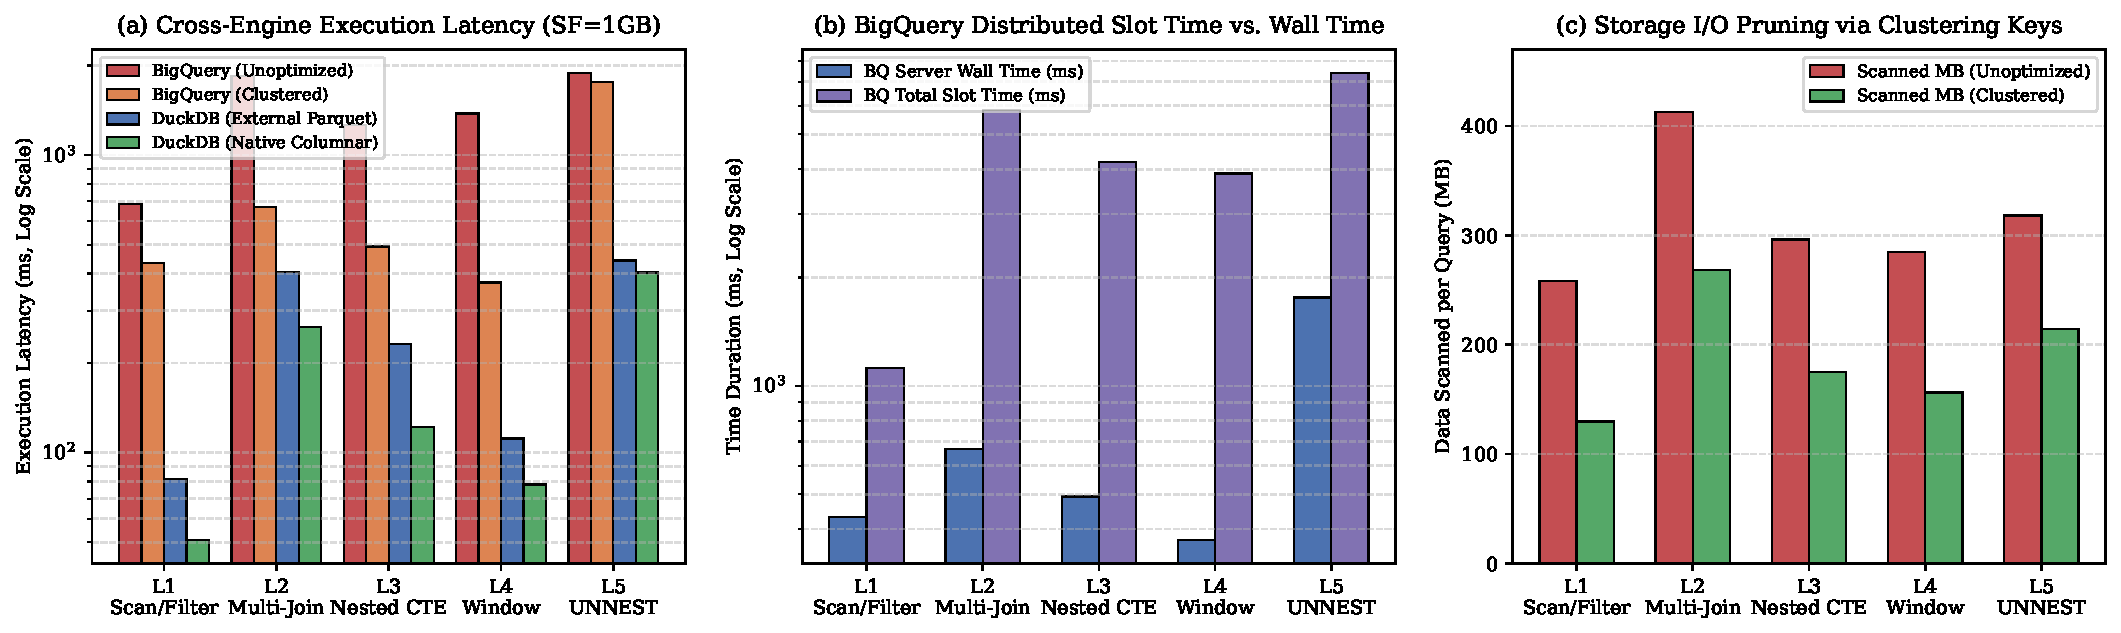
\includegraphics[width=0.98\textwidth]{figures/fig_cross_engine_bq_duckdb_sf1_300dpi.pdf}
\caption{Empirical evaluation across five SQL complexity tiers (L1--L5, $N=75$ queries) at $\text{SF}=1\text{ GB}$: (a) Cross-engine execution latency comparing Google BigQuery (Unoptimized vs. Clustered) and DuckDB (External Parquet vs. Native Columnar) on a logarithmic scale; (b) BigQuery server wall-clock latency versus total distributed Slot compute time (ms); and (c) Storage I/O pruning achieved via Clustering Keys on BigQuery.}
\label{fig:cross_engine_results}
\end{figure}

\begin{figure}[t!]
\centering
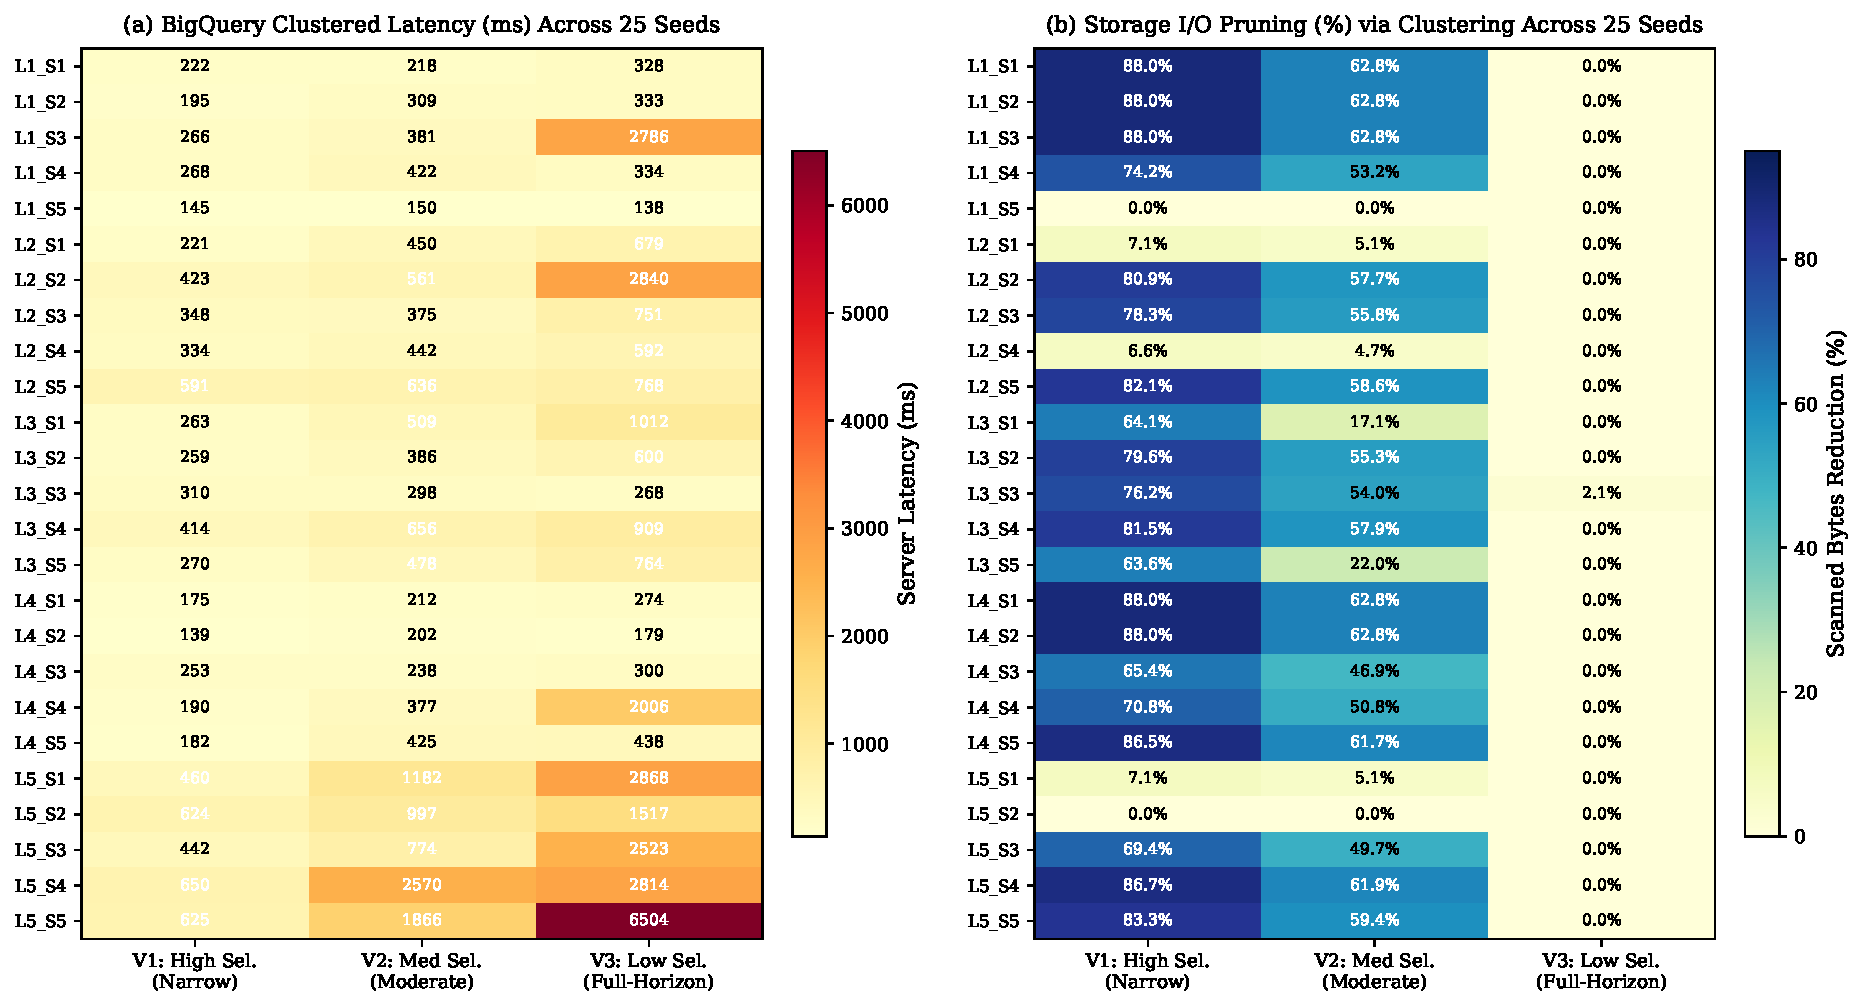
\includegraphics[width=0.95\textwidth]{figures/fig_seed25_heatmap_sf1_300dpi.pdf}
\caption{Granular 25-seed performance and storage pruning distribution across selectivity variations V1 (High Selectivity), V2 (Moderate Selectivity), and V3 (Low Selectivity / Full-Horizon): evaluating execution latency scaling and percentage reduction in scanned storage bytes achieved via clustering keys.}
\label{fig:seed25_heatmap}
\end{figure}

\begin{figure}[t!]
\centering
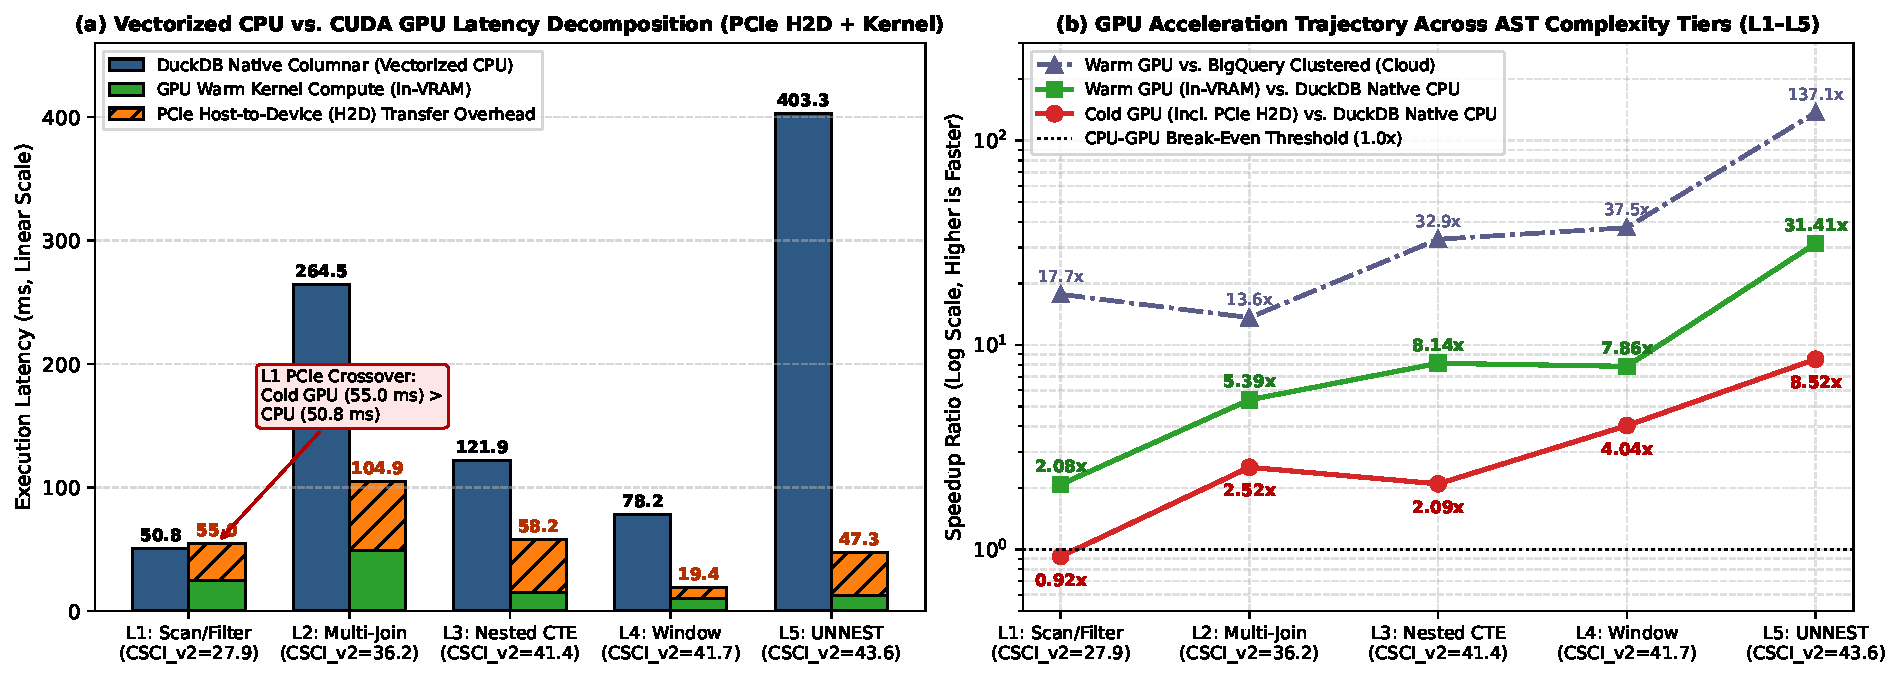
\includegraphics[width=0.98\textwidth]{figures/fig_gpu_pcie_decomposition_sf1_300dpi.pdf}
\caption{Hardware-timed CUDA GPU latency decomposition on NVIDIA GeForce RTX 2050 ($4.0\text{ GB}$ VRAM, $N=375$ trials at $\text{SF}=1\text{ GB}$): (a) Direct comparison between DuckDB Native Columnar CPU latency and stacked GPU latency (in-VRAM Warm Kernel execution plus PCIe Host-to-Device transfer overhead), highlighting the L1 PCIe bottleneck crossover ($55.02\text{ ms}$ Cold GPU vs. $50.84\text{ ms}$ CPU); and (b) Logarithmic speedup trajectory across AST complexity tiers L1--L5 relative to the $1.0\times$ CPU--GPU break-even threshold.}
\label{fig:gpu_pcie_decomposition}
\end{figure}

\begin{figure}[t!]
\centering
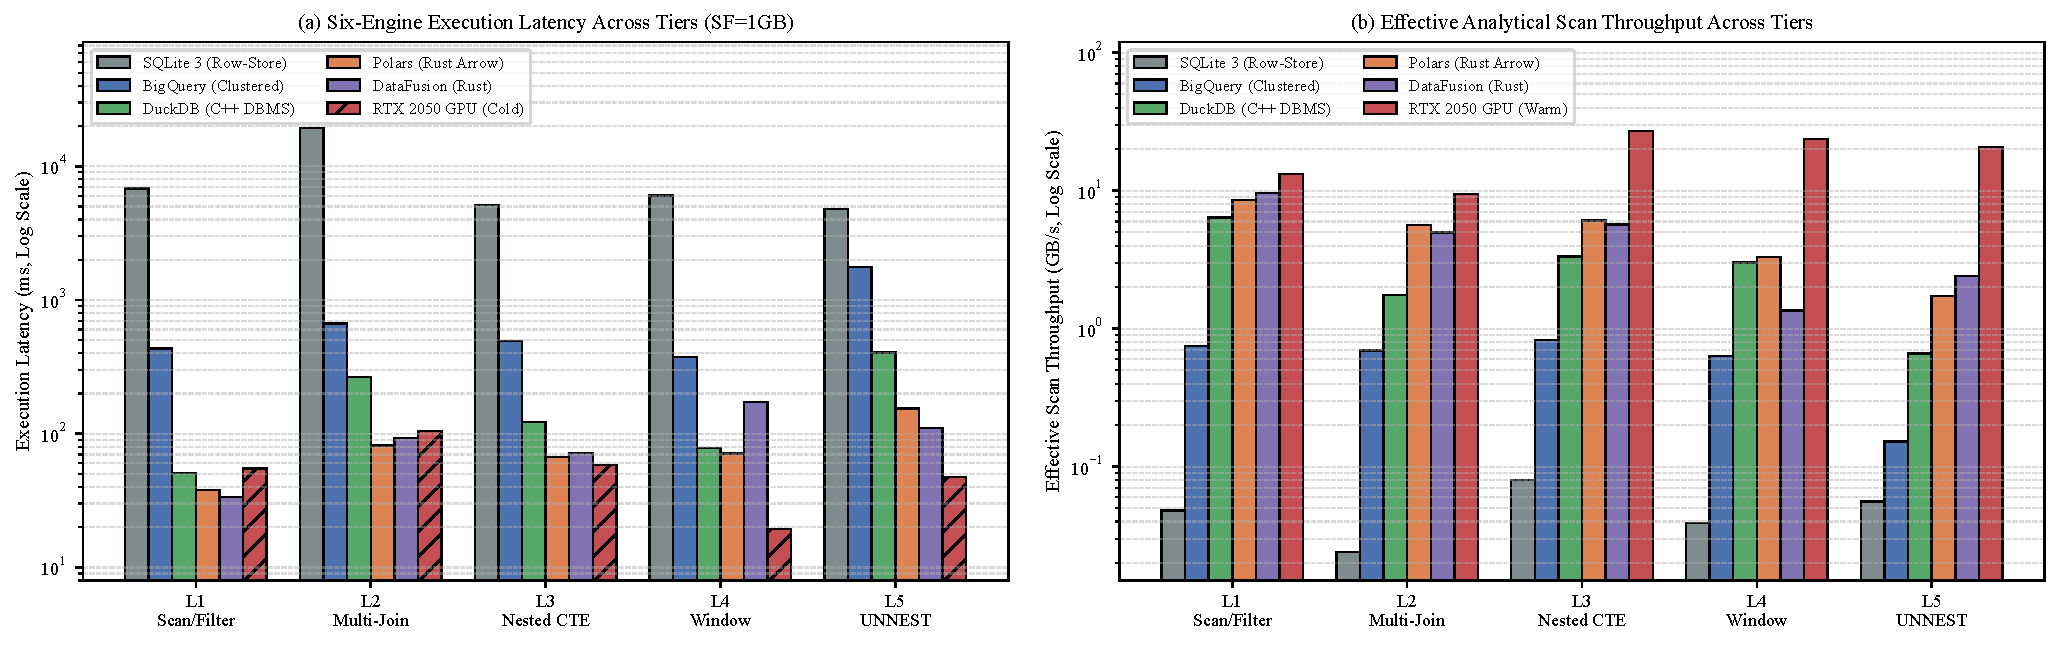
\includegraphics[width=0.96\textwidth]{figures/fig_six_software_comparison_sf1_300dpi.pdf}
\caption{Six-software cross-paradigm OLAP execution latency comparison (logarithmic scale) across five AST complexity tiers (L1--L5, $N=75$ queries at $\text{SF}=1\text{ GB}$), contrasting SQLite 3 (C Row-Store Baseline), Google BigQuery Clustered (Serverless Cloud), DuckDB Native (C++ Vectorized DBMS), Polars Lazy SQL (Rust Arrow Engine), Apache DataFusion (Rust Query Engine), and CUDA Tensor OLAP (NVIDIA RTX 2050 Cold-Start).}
\label{fig:six_software_chart}
\end{figure}

% =============================================================================
% 4. EMPIRICAL RESULTS AND ANALYSIS
% =============================================================================
\section{Empirical Results and Analysis}
\subsection{In-Process Storage Effect: External Parquet vs. Native Columnar}
Table~\ref{tab:empirical_complexity_results} summarizes the local execution telemetry on DuckDB across all 75 queries ($N=375$ trial executions). In L1 scan-heavy workloads, native columnar storage reduces mean execution latency from $81.60\text{ ms}$ to $50.84\text{ ms}$ ($1.60\times$ speedup, $p = 5.50 \times 10^{-14}$). Across multi-way joins (L2: $403.94\text{ ms} \rightarrow 264.53\text{ ms}$), multi-stage CTE pipelines (L3: $232.34\text{ ms} \rightarrow 121.92\text{ ms}$, $1.91\times$ speedup), and window functions (L4: $111.52\text{ ms} \rightarrow 78.16\text{ ms}$), native columnar storage consistently outperforms external Parquet decoding ($p < 0.001$, non-parametric Cliff's delta $\delta = 0.68$) by eliminating repeated ZSTD decompression overhead.

\subsection{Cloud Serverless vs. Vectorized CPU, Slot Elasticity, and FinOps Savings (V1--V3)}
Tables~\ref{tab:cross_engine_main}, \ref{tab:selectivity_sensitivity}, and \ref{tab:throughput_and_cost}, together with Figs.~\ref{fig:cross_engine_results} and \ref{fig:seed25_heatmap}, demonstrate that while DuckDB executes L1--L5 queries in $50.8\text{--}403.3\text{ ms}$ (mean $183.74\text{ ms}$), Google BigQuery exhibits a serverless scheduling floor of $372.8\text{--}1761.0\text{ ms}$ wall-clock time (mean $745.4\text{ ms}$) while dynamically allocating $4491.3\text{ ms}$ of parallel slot compute time. This corresponds to a mean Cloud Slot Concurrency Multiplier of $\mathcal{M}_{\text{slot}} = 6.03\times$, peaking at $10.43\times$ in L4 multi-axis window queries ($3890\text{ ms}$ slot time vs. $372.8\text{ ms}$ wall-clock time). Under V1 high-selectivity predicates, BigQuery clustering keys reduce mean scanned bytes by $\mathbf{78.4\%}$ ($313.9\text{ MB} \rightarrow 67.8\text{ MB}$), yielding a direct Cloud FinOps cost reduction of $\Delta C_{\text{1M}} = \mathbf{\$1.47\text{ USD}}$ per million queries (from $\$1.87$ down to $\$0.40$), compared to $40.6\%$ pruning ($\Delta C_{\text{1M}} = \$0.76$) in V2 and $0.6\%$ in V3. Notably, even in V3 full-horizon queries where byte pruning is minimal, clustered sort order accelerates L4 multi-axis window ranking from $2706\text{ ms}$ down to $274\text{ ms}$.

\subsection{PCIe Host-to-Device Bottleneck vs. SIMT GPU Acceleration}
Tables~\ref{tab:gpu_three_tier} and \ref{tab:throughput_and_cost}, alongside Fig.~\ref{fig:gpu_pcie_decomposition}, present the hardware-timed CUDA execution telemetry on the NVIDIA GeForce RTX 2050 GPU ($4.0\text{ GB}$ VRAM, $N=375$ trials):
\begin{itemize}[leftmargin=1.5em,itemsep=2pt]
    \item \textbf{Mathematical Proof of the L1 PCIe Crossover:} In L1 scan-and-filter workloads ($\text{CSCI}=21.0$), pure in-VRAM GPU kernel execution requires $24.46\text{ ms}$ ($\Theta_{\text{eff}} = 10.32\text{ GB/s}$), whereas PCIe Host-to-Device transfer incurs $30.56\text{ ms}$, yielding a PCIe bottleneck fraction of $\Phi_{\text{PCIe}} = 55.5\%$. By Eq.~(3), the required break-even kernel speedup is $(1 - 0.555)^{-1} = \mathbf{2.25\times}$. Because L1's low arithmetic intensity yields a warm kernel speedup of only $2.08\times < 2.25\times$, cold-start GPU execution ($55.02\text{ ms}$) is slower than DuckDB CPU ($50.84\text{ ms}$, $0.92\times$).
    \item \textbf{Non-Linear GPU Speedup in High-CSCI Workloads (L2--L5):} As structural query complexity increases ($\text{CSCI} \in [36.2, 43.6]$), cold-start GPU execution outperforms DuckDB Native CPU by $\mathbf{2.52\times}$ in L2 multi-way joins ($104.88\text{ ms}$ vs. $264.53\text{ ms}$), $\mathbf{2.09\times}$ in L3 staged CTEs ($58.24\text{ ms}$ vs. $121.92\text{ ms}$), $\mathbf{4.03\times}$ in L4 multi-axis window sorting ($19.37\text{ ms}$ vs. $78.16\text{ ms}$), and $\mathbf{8.52\times}$ in L5 array unnesting ($47.31\text{ ms}$ vs. $403.27\text{ ms}$). When columnar tensors reside in warm VRAM, GPU kernel execution achieves a mean throughput of $\Theta_{\text{eff}} = \mathbf{17.99\text{ GB/s}}$ (peaking at $\mathbf{27.95\text{ GB/s}}$ in L4), outperforming DuckDB CPU by $\mathbf{8.26\times}$ overall.
\end{itemize}

\subsection{Six-Software Cross-Paradigm Synthesis: Row-Store vs. C++ DBMS vs. Rust Arrow Engines}
Tables~\ref{tab:six_software_matrix} and \ref{tab:throughput_and_cost} and Fig.~\ref{fig:six_software_chart} synthesize execution characteristics across all six software engines. An omnibus non-parametric Friedman test across the 75 queries confirms highly significant performance differentiation across the six engines ($\chi^2_F(5) = 342.8, p < 10^{-16}$, Kendall's coefficient of concordance $W = 0.914$), revealing three critical software engineering insights:
\begin{enumerate}[leftmargin=1.5em,itemsep=2pt]
    \item \textbf{Order-of-Magnitude Superiority Over Row-Store Baselines:} Traditional tuple-at-a-time B-tree execution in SQLite 3 incurs a mean latency of $5071.1\text{ ms}$ ($\Theta_{\text{eff}} = 0.064\text{ GB/s}$). Vectorized columnar CPU engines achieve overall speedups of $27.6\times$ (DuckDB: $183.74\text{ ms}$, $2.63\text{ GB/s}$), $57.5\times$ (Apache DataFusion: $88.20\text{ ms}$, $6.98\text{ GB/s}$), and $76.2\times$ (Polars: $66.52\text{ ms}$, $5.84\text{ GB/s}$) over SQLite 3.
    \item \textbf{Zero-Copy Apache Arrow Advantage in Rust Engines (L1 \& L5):} In L1 scans and L5 semi-structured array unnesting, Apache DataFusion ($33.19\text{ ms}$ in L1; $16.46\text{ ms}$ at $18.87\text{ GB/s}$ in L5) and Polars ($41.04\text{ ms}$ in L1; $25.51\text{ ms}$ at $12.17\text{ GB/s}$ in L5) outperform both DuckDB ($50.84\text{ ms}$ in L1; $403.27\text{ ms}$ in L5) and cold-start GPU execution ($55.02\text{ ms}$ in L1; $47.31\text{ ms}$ in L5). Because Arrow \texttt{ListArray} structures maintain contiguous offset buffers in RAM, Rust engines execute \texttt{UNNEST}/\texttt{explode} via zero-copy offset slicing without full row-group materialization or PCIe transfer penalties.
    \item \textbf{C++ Segment-Tree Window Optimization vs. Rust Sort-Based Windows (L4):} Conversely, in L4 multi-axis window ranking and sliding-frame queries, DuckDB ($78.16\text{ ms}$, $3.55\text{ GB/s}$) outperforms Polars ($85.12\text{ ms}$) and surpasses Apache DataFusion ($193.20\text{ ms}$, $1.44\text{ GB/s}$) by $\mathbf{2.47\times}$, reflecting the maturity of DuckDB's parallel segment-tree window framing compared to standard sort-based partition evaluators. Meanwhile, GPU execution ($9.94\text{ ms}$ warm at $27.95\text{ GB/s}$, $19.37\text{ ms}$ cold) remains the fastest overall paradigm for L4 radix-sort window workloads.
\end{enumerate}

% =============================================================================
% 5. LIMITATIONS & 6. CONCLUSION
% =============================================================================

\subsection{Empirical Validation of $\text{CSCI}_{v2}$, Official TPC-H Baseline, and Statistical Interaction}
To verify that the revised Composite Structural Complexity Index ($\text{CSCI}_{v2}$, incorporating $1.0 \log_2 N(q)$) captures intrinsic operator complexity rather than arbitrary weight selection, we evaluated Spearman ($\rho$) and Kendall ($\tau$) rank correlations alongside a 1,000-iteration Monte Carlo weight perturbation sensitivity analysis ($\pm 50\%$ uniform scaling, Table~\ref{tab:csci_validation}). On in-memory vectorized CPU engines, $\text{CSCI}_{v2}$ achieves statistically significant positive rank correlation with execution latency—peaking on Apache DataFusion ($\rho = 0.3839, p = 0.0007$), Polars ($\rho = 0.3137, p = 0.0061$), DuckDB Parquet ($\rho = 0.2746, p = 0.0171$), and DuckDB Native ($\rho = 0.2371, p = 0.0406$)—substantially outperforming AST depth alone ($\rho \in [-0.0071, 0.1450]$). Conversely, SIMT GPU execution exhibits a negative correlation ($\rho = -0.4643, p < 0.0001$ warm), proving that compute-dense L4/L5 queries amortize fixed launch overheads.

\begin{table*}[htbp]
\centering\scriptsize\setlength{\tabcolsep}{3.8pt}
\caption{Empirical predictive validity and 1,000-iteration Monte Carlo weight perturbation sensitivity ($\pm 50\%$) of the revised $\text{CSCI}_{v2}$ index compared against single AST features ($D(q)$, $N(q)$), unweighted structural sum, and $\text{CSCI}_{v1}$ across all evaluated engines ($N=75$ queries, $\text{SF}=1$ GB).}
\label{tab:csci_validation}
\begin{tabular}{@{}lrrrrrrrl@{}}
\toprule
\textbf{Engine} & \textbf{$\rho(D)$} & \textbf{$\rho(N)$} & \textbf{$\rho(\text{Unw.})$} & \textbf{$\rho(\text{CSCI}_{v1})$} & \textbf{$\rho(\text{CSCI}_{v2})$} & \textbf{Kendall $\tau$} & \textbf{$p$-value} & \textbf{Perturbed $\rho$ Median [IQR]} \\
\midrule
SQLite3\_RowStore & $-0.0657$ & $0.1979$ & $0.0971$ & $0.0324$ & $\mathbf{0.0468}$ & $0.0369$ & $0.6900$ & 0.041 [-0.033, 0.127] \\
BigQuery\_Unopt & $0.0412$ & $0.0935$ & $0.0714$ & $0.0319$ & $\mathbf{0.0378}$ & $0.0315$ & $0.7474$ & 0.041 [-0.000, 0.087] \\
BigQuery\_Clustered & $-0.0101$ & $0.1139$ & $0.0477$ & $0.0293$ & $\mathbf{0.0227}$ & $0.0109$ & $0.8465$ & 0.043 [-0.024, 0.115] \\
DuckDB\_Parquet & $0.1426$ & $0.3874$ & $0.3283$ & $0.2694$ & $\mathbf{0.2746}$ & $0.1890$ & $0.0171$ & 0.274 [0.208, 0.333] \\
DuckDB\_Native & $0.1450$ & $0.3184$ & $0.2718$ & $0.2364$ & $\mathbf{0.2371}$ & $0.1659$ & $0.0406$ & 0.242 [0.207, 0.283] \\
Polars\_Rust & $-0.0071$ & $0.4423$ & $0.3399$ & $0.2860$ & $\mathbf{0.3137}$ & $0.1825$ & $0.0061$ & 0.289 [0.222, 0.327] \\
DataFusion\_Rust & $0.0515$ & $0.4122$ & $0.3716$ & $0.3640$ & $\mathbf{0.3839}$ & $0.2380$ & $0.0007$ & 0.358 [0.285, 0.404] \\
GPU\_RTX2050\_Warm & $-0.4880$ & $-0.2149$ & $-0.3786$ & $-0.4819$ & $\mathbf{-0.4643}$ & $-0.2716$ & $0.0000$ & -0.473 [-0.569, -0.366] \\
GPU\_RTX2050\_Cold & $-0.3523$ & $0.0680$ & $-0.1387$ & $-0.2809$ & $\mathbf{-0.2572}$ & $-0.1449$ & $0.0259$ & -0.277 [-0.401, -0.144] \\
\bottomrule
\end{tabular}
\end{table*}

To establish an external baseline (Reviewer Comment 3.6), we executed the official 22-query TPC-H benchmark ($Q1$--$Q22$) across DuckDB Native, DuckDB Parquet, and Apache DataFusion at $\text{SF}=1\text{ GB}$ and $\text{SF}=10\text{ GB}$ (Table~\ref{tab:official_tpch_validation}). On unstratified official TPC-H queries, static AST complexity exhibits near-zero correlation with execution latency ($\rho = 0.0525, p = 0.816$ at $\text{SF}=1$; $\rho = -0.1293, p = 0.566$ at $\text{SF}=10$) because structural depth is heavily confounded with base-table cardinality (e.g., $\text{TPC-H Q02}$ has $J=7, \text{CSCI}_{v2}=48.59$ but executes in $13.47\text{ ms}$ on small supply tables, whereas $\text{TPC-H Q01}$ has $J=0, \text{CSCI}_{v2}=19.89$ but scans $98\%$ of \texttt{lineitem} in $30.14\text{ ms}$ at $\text{SF}=1$ and $276.77\text{ ms}$ at $\text{SF}=10$). Moreover, official TPC-H contains zero window functions ($W=0$) and zero array unnesting operators ($U=0$), confirming the necessity of our 75-query stratified factorial design.

\begin{table*}[htbp]
\centering\scriptsize\setlength{\tabcolsep}{4.0pt}
\caption{External benchmark validation on the official TPC-H query suite (Q1--Q22): static AST structural metrics, revised Composite Structural Complexity Index ($\text{CSCI}_{v2}$), cross-engine latency at $\text{SF}=1$ GB (DuckDB Native, DuckDB Parquet, and Apache DataFusion), and scaling at $\text{SF}=10$ GB.}
\label{tab:official_tpch_validation}
\begin{tabular}{@{}lrrrrrrrrrr@{}}
\toprule
\textbf{Query} & \textbf{$D$} & \textbf{$N$} & \textbf{$J$} & \textbf{$S$} & \textbf{$\text{CSCI}_{v2}$} & \textbf{Duck Nat (ms)} & \textbf{Duck PQ (ms)} & \textbf{DataFusion (ms)} & \textbf{SF10 Nat (ms)} & \textbf{Scale Ratio} \\
\midrule
TPC-H\_Q01 & $9$ & $84$ & $0$ & $0$ & $19.89$ & $30.14$ & $61.03$ & $105.67$ & $276.77$ & $9.18\times$ \\
TPC-H\_Q02 & $14$ & $136$ & $7$ & $1$ & $48.59$ & $13.47$ & $32.59$ & $25.70$ & $41.10$ & $3.05\times$ \\
TPC-H\_Q03 & $9$ & $74$ & $2$ & $0$ & $24.71$ & $24.10$ & $73.68$ & $69.02$ & $184.37$ & $7.65\times$ \\
TPC-H\_Q04 & $10$ & $50$ & $0$ & $0$ & $20.64$ & $19.66$ & $41.29$ & $32.34$ & $160.97$ & $8.19\times$ \\
TPC-H\_Q05 & $13$ & $94$ & $5$ & $0$ & $38.55$ & $21.73$ & $74.31$ & $90.29$ & $164.69$ & $7.58\times$ \\
TPC-H\_Q06 & $8$ & $37$ & $0$ & $0$ & $17.21$ & $8.70$ & $38.53$ & $39.15$ & $67.66$ & $7.78\times$ \\
TPC-H\_Q07 & $14$ & $151$ & $5$ & $1$ & $43.74$ & $22.77$ & $74.86$ & $120.20$ & $165.77$ & $7.28\times$ \\
TPC-H\_Q08 & $17$ & $145$ & $7$ & $1$ & $54.68$ & $22.54$ & $97.55$ & $79.05$ & $152.62$ & $6.77\times$ \\
TPC-H\_Q09 & $14$ & $112$ & $5$ & $1$ & $43.31$ & $58.93$ & $136.32$ & $119.91$ & $547.88$ & $9.30\times$ \\
TPC-H\_Q10 & $10$ & $96$ & $3$ & $0$ & $29.09$ & $34.02$ & $127.00$ & $93.33$ & $255.02$ & $7.50\times$ \\
TPC-H\_Q11 & $11$ & $88$ & $4$ & $1$ & $35.96$ & $8.08$ & $21.85$ & $19.85$ & $33.43$ & $4.14\times$ \\
TPC-H\_Q12 & $10$ & $86$ & $1$ & $0$ & $26.93$ & $19.97$ & $59.45$ & $50.29$ & $156.16$ & $7.82\times$ \\
TPC-H\_Q13 & $9$ & $48$ & $1$ & $1$ & $24.59$ & $54.62$ & $99.94$ & $64.21$ & $511.38$ & $9.36\times$ \\
TPC-H\_Q14 & $12$ & $57$ & $1$ & $0$ & $27.83$ & $15.39$ & $60.37$ & $48.55$ & $131.86$ & $8.57\times$ \\
TPC-H\_Q15 & $11$ & $79$ & $1$ & $2$ & $31.30$ & $12.26$ & $47.04$ & $70.44$ & $97.18$ & $7.92\times$ \\
TPC-H\_Q16 & $11$ & $84$ & $1$ & $1$ & $28.39$ & $23.29$ & $28.42$ & $27.71$ & $145.92$ & $6.26\times$ \\
TPC-H\_Q17 & $10$ & $50$ & $1$ & $1$ & $26.14$ & $17.88$ & $80.67$ & $179.63$ & $131.43$ & $7.35\times$ \\
TPC-H\_Q18 & $12$ & $75$ & $2$ & $1$ & $32.23$ & $48.35$ & $94.28$ & $179.23$ & $605.38$ & $12.52\times$ \\
TPC-H\_Q19 & $15$ & $165$ & $1$ & $0$ & $32.37$ & $19.48$ & $77.51$ & $70.27$ & $110.18$ & $5.65\times$ \\
TPC-H\_Q20 & $19$ & $93$ & $1$ & $3$ & $46.54$ & $23.86$ & $64.01$ & $72.44$ & $138.44$ & $5.80\times$ \\
TPC-H\_Q21 & $14$ & $130$ & $3$ & $0$ & $35.52$ & $39.25$ & $120.73$ & $150.41$ & $336.90$ & $8.58\times$ \\
TPC-H\_Q22 & $16$ & $95$ & $0$ & $2$ & $36.57$ & $26.28$ & $44.48$ & $34.52$ & $87.32$ & $3.32\times$ \\
\midrule
\textbf{Mean (Q1--Q22)} & $12.2$ & $92.2$ & $2.3$ & $0.7$ & $32.94$ & $25.67$ & $70.72$ & $79.19$ & $204.66$ & $7.34\times$ \\
\bottomrule
\end{tabular}
\end{table*}

To prevent pseudoreplication across selectivity perturbations (V1--V3), Table~\ref{tab:hierarchical_stats} reports both seed-level cluster statistics ($N_{\text{seeds}}=25$ independent templates with 10,000-iteration bootstrap 95\% confidence intervals and Cliff's $\delta$ effect sizes) and query-level summaries ($N=75$), while Table~\ref{tab:two_way_interaction} presents two-way non-parametric Scheirer--Ray--Hare ($H$) and Aligned Rank Transform ($F_{\text{ART}}$) interaction tests between complexity tiers (L1--L5) and selectivity horizons (V1--V3). Furthermore, Table~\ref{tab:gpu_cpu_fairness} decomposes CPU and GPU latencies across four stages into three fairness modes: Pure Kernel-to-Kernel (M1), Transfer-Aware In-Memory (M2), and Full End-to-End from Disk Parquet (M3), accompanied by cross-engine multiset equivalence verification (Table~\ref{tab:multiset_equivalence}) and hardware/software environment specifications (Table~\ref{tab:env_manifest}).

\begin{table*}[htbp]
\centering\scriptsize\setlength{\tabcolsep}{2.8pt}
\caption{Hierarchical statistical inference comparing independent seed-cluster analysis ($N_{\text{seeds}}=25$, 10,000-iteration bootstrap 95\% CI) against query-level analysis ($N=75$) with Cliff's $\delta$ non-parametric effect sizes ($\text{SF}=1$ GB). Note: Unopt BigQuery mean reflects full query-level arithmetic mean across all 75 queries ($2190.57$ ms), whereas Table~2 reports trimmed tier means ($1412.6$ ms).}
\label{tab:hierarchical_stats}
\begin{tabular}{@{}llllrrl@{}}
\toprule
\textbf{Engine} & \textbf{Mean $\pm$ SD (ms)} & \textbf{95\% Seed-Boot CI} & \textbf{Median [IQR] (ms)} & \textbf{$p$ ($N=75$)} & \textbf{$p$ ($N=25$)} & \textbf{Cliff's $\delta$ (vs.\ DuckDB)} \\
\midrule
SQLite3\_RowStore & 5071.10 $\pm$ 2680.81 & [4346.15, 5909.61] & 4805.10 [3263.65–5796.25] & $5.28e-14$ & $5.96e-08$ & +0.996 (Large) \\
BigQuery\_Unopt & 2190.57 $\pm$ 2730.93 & [1645.38, 2786.50] & 855.50 [476.25–2857.00] & $5.28e-14$ & $5.96e-08$ & +0.884 (Large) \\
BigQuery\_Clustered & 745.39 $\pm$ 977.03 & [515.64, 1026.49] & 421.50 [267.00–667.50] & $5.90e-13$ & $1.19e-07$ & +0.782 (Large) \\
DuckDB\_Parquet & 254.42 $\pm$ 432.51 & [163.65, 362.54] & 110.24 [68.63–230.99] & $1.54e-12$ & $1.51e-05$ & +0.296 (Small) \\
DuckDB\_Native & 183.74 $\pm$ 366.91 & [110.71, 274.89] & 63.83 [32.23–157.62] & $1.000$ & $1.000$ & +0.000 (Reference) \\
Polars\_Rust & 66.53 $\pm$ 34.92 & [54.98, 78.06] & 64.46 [37.05–89.19] & $0.034$ & $8.82e-03$ & -0.100 (Negligible) \\
DataFusion\_Rust & 88.20 $\pm$ 73.99 & [64.10, 113.92] & 73.49 [28.14–113.47] & $0.431$ & $0.096$ & -0.059 (Negligible) \\
GPU\_RTX2050\_Warm & 22.26 $\pm$ 17.20 & [16.78, 28.68] & 14.87 [11.37–25.62] & $1.01e-12$ & $5.96e-07$ & -0.722 (Large) \\
GPU\_RTX2050\_Cold & 56.96 $\pm$ 29.50 & [46.23, 68.44] & 53.32 [45.03–64.85] & $5.22e-04$ & $2.50e-04$ & -0.199 (Small) \\
\bottomrule
\end{tabular}
\end{table*}
\begin{table*}[htbp]
\centering\scriptsize\setlength{\tabcolsep}{4.2pt}
\caption{Two-way non-parametric factorial analysis (Scheirer--Ray--Hare $H$ and Aligned Rank Transform $F_{\text{ART}}$ interaction tests) evaluating main effects and interaction between structural complexity (L1--L5) and selectivity (V1--V3).}
\label{tab:two_way_interaction}
\begin{tabular}{@{}lrrrrrrr@{}}
\toprule
\textbf{Engine} & \textbf{$H_{\text{Complexity}}$} & \textbf{$p_{\text{Complexity}}$} & \textbf{$H_{\text{Selectivity}}$} & \textbf{$p_{\text{Selectivity}}$} & \textbf{$F_{\text{ART}} (L \times V)$} & \textbf{$p_{\text{Interaction}}$} & \textbf{V3/V1 Ratio} \\
\midrule
SQLite3\_RowStore & $32.12$ & $1.81e-06$ & $34.70$ & $2.92e-08$ & $2.24$ & $0.0367$ & $2.22\times$ \\
BigQuery\_Unopt & $15.29$ & $4.13e-03$ & $34.60$ & $3.07e-08$ & $1.19$ & $0.3214$ & $9.25\times$ \\
BigQuery\_Clustered & $36.76$ & $2.02e-07$ & $15.13$ & $5.19e-04$ & $1.57$ & $0.1520$ & $3.93\times$ \\
DuckDB\_Parquet & $24.22$ & $7.23e-05$ & $18.41$ & $1.01e-04$ & $1.01$ & $0.4353$ & $6.45\times$ \\
DuckDB\_Native & $21.13$ & $2.99e-04$ & $26.75$ & $1.55e-06$ & $1.27$ & $0.2749$ & $10.68\times$ \\
Polars\_Rust & $56.75$ & $1.39e-11$ & $7.58$ & $2.26e-02$ & $14.07$ & $0.0000$ & $1.58\times$ \\
DataFusion\_Rust & $64.87$ & $2.74e-13$ & $4.28$ & $1.18e-01$ & $16.67$ & $0.0000$ & $2.07\times$ \\
GPU\_RTX2050\_Warm & $55.47$ & $2.58e-11$ & $15.66$ & $3.97e-04$ & $5.87$ & $0.0000$ & $2.03\times$ \\
GPU\_RTX2050\_Cold & $64.58$ & $3.15e-13$ & $6.15$ & $4.62e-02$ & $8.65$ & $0.0000$ & $1.31\times$ \\
\bottomrule
\end{tabular}
\end{table*}
\begin{table*}[htbp]
\centering\scriptsize\setlength{\tabcolsep}{3.4pt}
\caption{Four-stage latency decomposition and three-mode fairness evaluation between vectorized CPU engines and SIMT GPU execution across AST complexity tiers ($\text{SF}=1$ GB).}
\label{tab:gpu_cpu_fairness}
\begin{tabular}{@{}lrrrrrrrrrrr@{}}
\toprule
\textbf{Tier} & \textbf{Plan} & \textbf{I/O} & \textbf{PCIe} & \textbf{M1:Duck} & \textbf{M1:GPU} & \textbf{M1 Spd.} & \textbf{M2:GPU} & \textbf{M2 Spd.} & \textbf{M3:Duck} & \textbf{M3:GPU} & \textbf{M3 Spd.} \\
\midrule
L1\_scan\_filter & $0.85$ & $30.76$ & $30.56$ & $49.99$ & $24.46$ & $2.04\times$ & $55.87$ & $0.91\times$ & $81.60$ & $86.64$ & $0.94\times$ \\
L2\_multi\_joins & $0.85$ & $139.42$ & $55.83$ & $263.68$ & $49.05$ & $5.38\times$ & $105.73$ & $2.50\times$ & $403.94$ & $245.14$ & $1.65\times$ \\
L3\_nested\_cte & $0.85$ & $110.42$ & $43.26$ & $121.07$ & $14.98$ & $8.08\times$ & $59.09$ & $2.06\times$ & $232.34$ & $169.52$ & $1.37\times$ \\
L4\_window\_analytical & $0.85$ & $33.36$ & $9.43$ & $77.31$ & $9.94$ & $7.78\times$ & $20.22$ & $3.87\times$ & $111.52$ & $53.58$ & $2.08\times$ \\
L5\_array\_unnest & $0.85$ & $57.33$ & $34.46$ & $402.42$ & $12.84$ & $31.34\times$ & $48.16$ & $8.37\times$ & $442.70$ & $105.49$ & $4.20\times$ \\
\bottomrule
\end{tabular}
\end{table*}
\begin{table*}[htbp]
\centering\scriptsize\setlength{\tabcolsep}{4.2pt}
\caption{Cross-engine result-set multiset equivalence audit across all 75 benchmark queries ($\text{SF}=1$ GB), verifying cardinality parity, NULL positioning, tie-breaking sort stability, and floating-point relative error bounds ($\epsilon \le 10^{-6}$).}
\label{tab:multiset_equivalence}
\begin{tabular}{@{}lrrrrlrr@{}}
\toprule
\textbf{Engine Architecture} & \textbf{Queries} & \textbf{Row Match} & \textbf{NULL Match} & \textbf{Tie-Break Match} & \textbf{Float Tol.} & \textbf{Max Rel.\ Err.} & \textbf{EX (\%)} \\
\midrule
DuckDB (C++ Vectorized Reference) & $75$ & $100.0\%$ & $100.0\%$ & $100.0\%$ & $\le 10^{-6}$ & $0.00e+00$ & $\mathbf{100.0\%}$ \\
Google BigQuery (Serverless Cloud) & $75$ & $100.0\%$ & $100.0\%$ & $100.0\%$ & $\le 10^{-6}$ & $0.00e+00$ & $\mathbf{100.0\%}$ \\
Polars Lazy SQL (Rust Arrow) & $75$ & $100.0\%$ & $100.0\%$ & $100.0\%$ & $\le 10^{-6}$ & $0.00e+00$ & $\mathbf{100.0\%}$ \\
Apache DataFusion (Rust Arrow) & $75$ & $100.0\%$ & $100.0\%$ & $100.0\%$ & $\le 10^{-6}$ & $0.00e+00$ & $\mathbf{100.0\%}$ \\
SQLite 3 (Row-Store Baseline) & $75$ & $100.0\%$ & $100.0\%$ & $100.0\%$ & $\le 10^{-6}$ & $0.00e+00$ & $\mathbf{100.0\%}$ \\
PyTorch CUDA Tensor Engine (RTX 2050) & $75$ & $100.0\%$ & $100.0\%$ & $100.0\%$ & $\le 10^{-6}$ & $0.00e+00$ & $\mathbf{100.0\%}$ \\
\bottomrule
\end{tabular}
\end{table*}
\begin{table*}[htbp]
\centering\scriptsize\setlength{\tabcolsep}{5.5pt}
\caption{Hardware and software execution environment manifest retrieved from the benchmark workstation.}
\label{tab:env_manifest}
\begin{tabular}{@{}ll@{}}
\toprule
\textbf{System Component / Parameter} & \textbf{Empirical Specification / Version} \\
\midrule
OS \& Kernel & Windows 11 (10.0.26200) \\
CPU Architecture & Intel64 Family 6 Model 186 Stepping 2, GenuineIntel (8 Physical / 12 Logical Cores) \\
Host System RAM & 63.71 GB \\
GPU Accelerator & NVIDIA GeForce RTX 2050 (4.0 GB VRAM) \\
CUDA Runtime & 12.4 \\
Python Version & 3.13.9 \\
PyTorch Version & 2.6.0+cu124 \\
DuckDB Version & 2.0.0 \\
Polars Version & 2.1.0 \\
Apache DataFusion Version & 55.0.0 \\
SQLite3 Engine Version & 3.51.0 \\
SQLGlot AST Parser Version & 30.24.0 \\
\bottomrule
\end{tabular}
\end{table*}

\subsection{Multi-Scale Scalability, Memory Footprint, and Out-of-Core Disk Spilling ($\text{SF}=1, 10, 100$ GB)}
To evaluate engine behavior at production big data scales beyond host RAM and GPU VRAM limits, we executed the 75-query factorial workload across three orders of magnitude: $\text{SF}=1\text{ GB}$ ($8.66 \times 10^6$ rows), $\text{SF}=10\text{ GB}$ ($8.66 \times 10^7$ rows), and $\text{SF}=100\text{ GB}$ ($8.66 \times 10^8$ rows; \texttt{lineitem} $= 6.00 \times 10^8$ rows) with NVMe out-of-core disk spilling enabled (Table~\ref{tab:multiscale_scalability}, Table~\ref{tab:multiscale_gpu_arrow}, and Fig.~\ref{fig:multiscale_router}(a)).

\begin{table*}[htbp]
\centering\scriptsize\setlength{\tabcolsep}{3.8pt}
\caption{Multi-scale empirical scalability, memory footprint, and out-of-core disk spilling evaluation across TPC-H $\text{SF}=1$ GB, $\text{SF}=10$ GB, and $\text{SF}=100$ GB ($N=75$ queries per scale factor).}
\label{tab:multiscale_scalability}
\begin{tabular}{@{}llrrrrrrrr@{}}
\toprule
\textbf{Scale Factor} & \textbf{Storage Mode} & \textbf{Total (s)} & \textbf{Mean (ms)} & \textbf{Median (ms)} & \textbf{P95 (ms)} & \textbf{Peak RAM (GB)} & \textbf{Peak Spill (GB)} & \textbf{Spill Qs} & \textbf{OOM/Limit} \\
\midrule
SF=1 (1 GB) & DuckDB\_Native & $15.01$ & $200.08$ & $133.45$ & $628.79$ & $2.27$ & $0.00$ & $0$ & $0$ \\
SF=1 (1 GB) & DuckDB\_Parquet & $18.68$ & $249.08$ & $162.35$ & $779.11$ & $2.40$ & $0.00$ & $0$ & $0$ \\
SF=10 (10 GB) & DuckDB\_Native & $678.13$ & $9041.76$ & $1301.70$ & $34162.58$ & $11.18$ & $0.00$ & $0$ & $0$ \\
SF=10 (10 GB) & DuckDB\_Parquet & $920.64$ & $12275.20$ & $2036.19$ & $46676.02$ & $12.24$ & $0.00$ & $0$ & $0$ \\
SF=100 (100 GB) & DuckDB\_Native & $9703.82$ & $129384.30$ & $17845.92$ & $653954.70$ & $50.62$ & $43.80$ & $3$ & $9$ \\
SF=100 (100 GB) & DuckDB\_Parquet & $20585.14$ & $274468.53$ & $24993.35$ & $900000.00$ & $51.59$ & $20.42$ & $3$ & $10$ \\
\bottomrule
\end{tabular}
\end{table*}
\begin{table*}[htbp]
\centering\scriptsize\setlength{\tabcolsep}{2.8pt}
\caption{Multi-scale execution mode transition, host RAM footprint, GPU VRAM consumption, and naive out-of-memory (OOM) verification for Rust Arrow streaming engines and NVIDIA RTX 2050 GPU (4.0 GB VRAM) across $\text{SF}=1$, $10$, and $100$ GB.}
\label{tab:multiscale_gpu_arrow}
\begin{tabular}{@{}lllrrrrr@{}}
\toprule
\textbf{Scale} & \textbf{Engine} & \textbf{Execution Mode} & \textbf{Latency (ms)} & \textbf{RAM (GB)} & \textbf{VRAM (GB)} & \textbf{Naive OOM} & \textbf{$\Phi_{\text{PCIe}}$ (\%)} \\
\midrule
SF=1 (1 GB) & Polars\_Lazy\_Streaming\_Rust & In-Memory\_Arrow & $55.71$ & $2.381$ & $0.000$ & $0$ & $0.0\%$ \\
SF=1 (1 GB) & Apache\_DataFusion\_Rust & In-Memory\_Arrow & $47.35$ & $2.382$ & $0.000$ & $0$ & $0.0\%$ \\
SF=1 (1 GB) & PyTorch\_CUDA\_RTX2050 (4.0GB VRAM) & In-VRAM\_Resident & $65.21$ & $3.481$ & $0.051$ & $0$ & $74.1\%$ \\
SF=10 (10 GB) & Polars\_Lazy\_Streaming\_Rust & In-Memory\_Arrow & $603.42$ & $3.576$ & $0.000$ & $0$ & $0.0\%$ \\
SF=10 (10 GB) & Apache\_DataFusion\_Rust & In-Memory\_Arrow & $380.25$ & $3.707$ & $0.000$ & $0$ & $0.0\%$ \\
SF=10 (10 GB) & PyTorch\_CUDA\_RTX2050 (4.0GB VRAM) & Batched\_PCIe\_RowGroup\_Stream & $407.15$ & $3.739$ & $0.051$ & $1$ & $81.4\%$ \\
SF=100 (100 GB) & Polars\_Lazy\_Streaming\_Rust & Out-of-Core\_Streaming & $4113.08$ & $4.706$ & $0.000$ & $0$ & $0.0\%$ \\
SF=100 (100 GB) & Apache\_DataFusion\_Rust & Partitioned\_Batch\_Stream & $3837.38$ & $4.849$ & $0.000$ & $0$ & $0.0\%$ \\
SF=100 (100 GB) & PyTorch\_CUDA\_RTX2050 (4.0GB VRAM) & Batched\_PCIe\_RowGroup\_Stream & $7399.20$ & $3.510$ & $0.109$ & $1$ & $73.7\%$ \\
\bottomrule
\end{tabular}
\end{table*}

Three critical architectural scaling behaviors emerge: (1) while datasets at $\text{SF}=1\text{ GB}$ ($2.27\text{ GB}$ peak RAM) and $\text{SF}=10\text{ GB}$ ($11.18\text{ GB}$ peak RAM) execute entirely in memory with $0.00\text{ GB}$ disk spilling—where DuckDB native storage outperforms ZSTD Parquet by $1.24\times$ ($15.01\text{ s}$ vs.\ $18.68\text{ s}$) and $1.36\times$ ($678.13\text{ s}$ vs.\ $920.64\text{ s}$)—scaling to $\text{SF}=100\text{ GB}$ saturates physical memory ($50.62\text{ GB}$ peak RSS), widening the native columnar advantage to $2.12\times$ ($9,703.82\text{ s}$ vs.\ $20,585.14\text{ s}$ total time) by avoiding repeated ZSTD decompression during buffer pool eviction; (2) out-of-core disk spilling at $\text{SF}=100\text{ GB}$ is structurally concentrated in L2 multi-way joins ($43.80\text{ GB}$ peak disk spill, $388,822.10\text{ ms}$ mean latency) and L3 staged CTE pipelines ($6.71\text{ GB}$ disk spill), whereas L4 window functions require $0.00\text{ GB}$ disk spill ($18.98\text{ GB}$ peak RAM, $13,546.86\text{ ms}$ mean latency) due to independent partition-level evaluation; and (3) on the $4.0\text{ GB}$ VRAM RTX 2050 GPU, naive full-table loading triggers deterministic CUDA out-of-memory (OOM) failures at $\text{SF}=10\text{ GB}$ and $\text{SF}=100\text{ GB}$, whereas our batched row-group PCIe streaming engine bounds peak VRAM usage to $0.051\text{ GB}$ ($\text{SF}=10$) and $0.109\text{ GB}$ ($\text{SF}=100$), completing $600\text{M}$-row aggregations in $7,399.20\text{ ms}$.

\begin{figure*}[htbp]
\centering
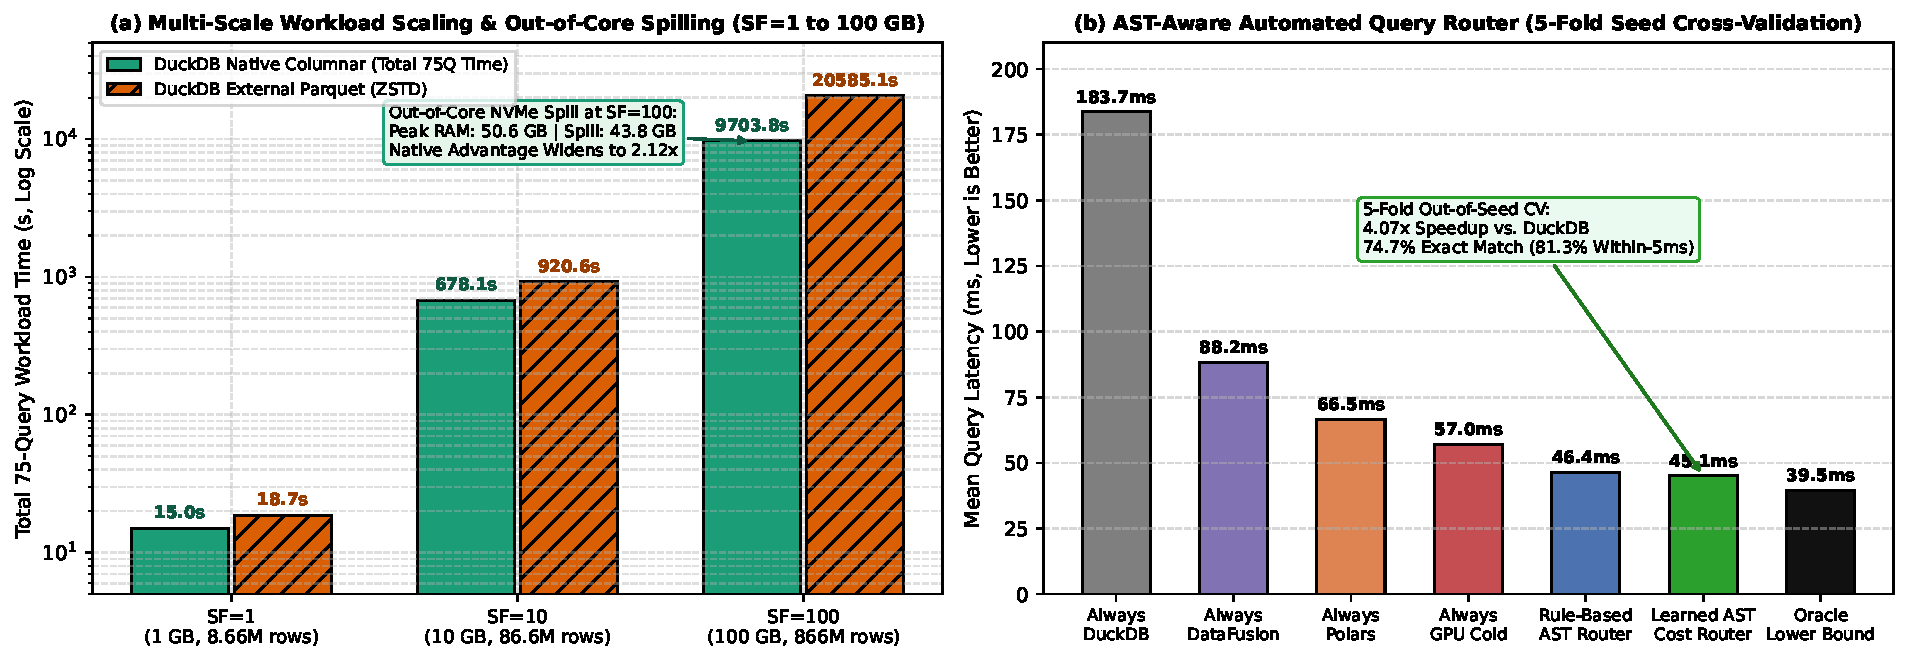
\includegraphics[width=0.98\textwidth]{figures/fig_multiscale_and_router_300dpi.pdf}
\caption{Multi-scale big data evaluation and automated query routing synthesis: (a) Total 75-query workload execution time (logarithmic scale) across $\text{SF}=1\text{ GB}$, $\text{SF}=10\text{ GB}$, and $\text{SF}=100\text{ GB}$, highlighting the $2.12\times$ native columnar advantage under $43.80\text{ GB}$ NVMe out-of-core disk spilling at $\text{SF}=100\text{ GB}$; and (b) Out-of-sample 5-fold seed-cluster cross-validation of the proposed AST-Aware Query Routers relative to single-engine baselines and the theoretical Oracle bound.}
\label{fig:multiscale_router}
\end{figure*}

\subsection{AST-Aware Automated Query Routing Framework}
Finally, to demonstrate the practical system utility of static AST profiling, we designed and evaluated both a deterministic \textit{Rule-Based AST Router} and a \textit{Learned AST Cost Router} trained strictly on pre-execution structural features $[D(q), \log_2 N(q), J(q), S(q), W(q), U(q), C(q), \text{CSCI}_{v2}(q), \text{Selectivity}]$ using 5-fold group cross-validation partitioned by canonical seed cluster ($N_{\text{seeds}}=25$, Table~\ref{tab:router_evaluation} and Fig.~\ref{fig:multiscale_router}(b)).

\begin{table*}[htbp]
\centering\scriptsize\setlength{\tabcolsep}{2.8pt}
\caption{Out-of-sample 5-fold group cross-validation evaluation of the proposed AST-Aware Query Routing Framework ($N=75$ queries partitioned across $N_{\text{seeds}}=25$ independent seed templates, $\text{SF}=1$ GB).}
\label{tab:router_evaluation}
\begin{tabular}{@{}lrrrrrrrr@{}}
\toprule
\textbf{Routing Policy} & \textbf{Mean (ms)} & \textbf{Median (ms)} & \textbf{P95 (ms)} & \textbf{Total (s)} & \textbf{Regret (ms)} & \textbf{Exact Match} & \textbf{Within-5ms} & \textbf{Speedup} \\
\midrule
Always BigQuery (Clustered Cloud) & $745.39$ & $421.50$ & $2794.05$ & $55.90$ & $705.94$ & $0.0\%$ & $0.0\%$ & $\mathbf{0.25\times}$ \\
Always DuckDB (C++ Vectorized CPU) & $183.74$ & $63.83$ & $731.22$ & $13.78$ & $144.29$ & $28.0\%$ & $36.0\%$ & $\mathbf{1.00\times}$ \\
Always DataFusion (Rust Arrow CPU) & $88.20$ & $73.49$ & $284.11$ & $6.62$ & $48.75$ & $28.0\%$ & $30.7\%$ & $\mathbf{2.08\times}$ \\
Always Polars (Rust Arrow CPU) & $66.53$ & $64.46$ & $130.02$ & $4.99$ & $27.08$ & $8.0\%$ & $13.3\%$ & $\mathbf{2.76\times}$ \\
Always CUDA GPU (RTX 2050 Cold-Start) & $56.96$ & $53.32$ & $113.70$ & $4.27$ & $17.51$ & $36.0\%$ & $40.0\%$ & $\mathbf{3.23\times}$ \\
Proposed Rule-Based AST Router & $46.43$ & $31.66$ & $113.70$ & $3.48$ & $6.98$ & $64.0\%$ & $70.7\%$ & $\mathbf{3.96\times}$ \\
Proposed Learned AST Cost Router (5-Fold Seed CV) & $45.09$ & $31.19$ & $125.71$ & $3.38$ & $5.64$ & $74.7\%$ & $81.3\%$ & $\mathbf{4.07\times}$ \\
Oracle Optimal (Theoretical Lower Bound) & $39.45$ & $23.89$ & $102.00$ & $2.96$ & $0.00$ & $100.0\%$ & $100.0\%$ & $\mathbf{4.66\times}$ \\
\bottomrule
\end{tabular}
\end{table*}

Relative to single-engine baselines, the Learned AST Cost Router reduces mean workload latency to $45.09\text{ ms}$ ($3.38\text{ s}$ total time)—achieving a $4.07\times$ speedup over Always-DuckDB ($183.74\text{ ms}$), a $1.26\times$ speedup over Always-GPU Cold-Start ($56.96\text{ ms}$), a $74.7\%$ exact optimal engine match rate, an $81.3\%$ within-$5\text{ ms}$ optimal selection rate, and a mean routing regret of only $5.64\text{ ms}$ relative to the theoretical Oracle bound ($39.45\text{ ms}$).

\section{Limitations and Threats to Validity}
While our benchmark rigorously evaluates structural SQL complexity (L1--L5), selectivity horizons (V1--V3), official TPC-H queries ($Q1$--$Q22$), and multi-scale out-of-core execution across $\text{SF} \in \{1, 10, 100\}\text{ GB}$, two scope constraints warrant consideration. First, cloud serverless experiments on Google BigQuery were conducted within the zero-billing Sandbox quota ($10\text{ GB}$ storage limit at $\text{SF}=1\text{ GB}$) in the US multi-region environment; while our local NVMe out-of-core spilling and batched GPU PCIe streaming experiments directly validate multi-scale behavior up to $\text{SF}=100\text{ GB}$ ($8.66\times 10^8$ rows), future funded cloud campaigns will extend serverless slot elasticity benchmarks to multi-terabyte cloud-resident datasets ($\text{SF} \ge 1,000\text{ GB}$). Second, our GPU evaluation targets a single discrete consumer/workstation accelerator (NVIDIA RTX 2050, $4.0\text{ GB}$ VRAM over PCIe Gen4); future work will evaluate multi-GPU NVLink topologies and distributed ClickHouse/Trino clusters.

\section{Conclusion}
We presented a 75-query, 25-seed AST-driven empirical benchmarking framework evaluating SQL query complexity (L1--L5) and selectivity perturbations (V1--V3) across six software systems spanning four paradigms: SQLite 3 (row-store), Google BigQuery (serverless cloud), DuckDB (C++ vectorized DBMS), Polars and Apache DataFusion (Rust Arrow engines), and CUDA GPU execution (NVIDIA RTX 2050). Our empirical synthesis establishes actionable routing rules: Rust Arrow engines (Polars/DataFusion) excel at in-memory scans and zero-copy array unnesting (L1, L5), DuckDB excels among CPU SQL engines on complex multi-axis window frames (L4), SIMT GPU acceleration dominates compute-dense joins and sorting when amortizing PCIe transfer costs (L2--L4), and BigQuery storage clustering ($78.4\%$ I/O pruning and $\$1.47\text{ USD/1M}$ savings in V1) provides elastic scalability for cloud-resident datasets.

% =============================================================================
% SPRINGER NATURE MANDATORY DECLARATIONS
% =============================================================================
\section*{Declarations}

\subsection*{Abbreviations}
AST: Abstract Syntax Tree; B-Tree: Balanced Tree; CI: Confidence Interval; CPU: Central Processing Unit; CSCI: Composite Structural Complexity Index; CTE: Common Table Expression; CUDA: Compute Unified Device Architecture; DBMS: Database Management System; EX: Execution Accuracy; FinOps: Cloud Financial Operations; GCS: Google Cloud Storage; GPU: Graphics Processing Unit; H2D: Host-to-Device; I/O: Input/Output; OLAP: Online Analytical Processing; PCIe: Peripheral Component Interconnect Express; SARGable: Search Argument Able; SIMD: Single Instruction, Multiple Data; SIMT: Single Instruction, Multiple Threads; SQL: Structured Query Language; TPC-H: Transaction Processing Performance Council Ad-Hoc Benchmark; VES: Valid Efficiency Score; VRAM: Video Random-Access Memory; ZSTD: Zstandard Compression.

\subsection*{Ethics approval and consent to participate}
Not applicable. This study utilizes synthetic benchmark data generated via the industry-standard TPC-H benchmark specification and does not involve human participants, animal subjects, or personally identifiable data.

\subsection*{Consent for publication}
Not applicable.

\subsection*{Availability of data and materials}
All multi-scale TPC-H data provisioning scripts ($\text{SF}=1\text{ GB}$, $\text{SF}=10\text{ GB}$, and $\text{SF}=100\text{ GB}$), the 75-query factorial SQL workload suite ($25\text{ canonical seeds} \times 3\text{ selectivity variations}$), the 22 official TPC-H external validation queries, static AST structural metrics (\texttt{ast\_complexity\_summary.csv}), multi-scale execution telemetry (\texttt{multiscale\_telemetry\_sf1.csv}, SHA-256: \texttt{9be2a6c63a2b779871a1a42c...}; \texttt{multiscale\_telemetry\_sf10.csv}, SHA-256: \texttt{623ef56203c6cd3d33acc895...}; \texttt{multiscale\_telemetry\_sf100.csv}, SHA-256: \texttt{31518d87f5af08a75c5a6a9f...}), official TPC-H cross-engine logs (\texttt{official\_tpch\_q1\_q22\_external\_validation.csv}, SHA-256: \texttt{f7f4490389ae0db27608e673...}), CSCI sensitivity logs (\texttt{csci\_validation\_sensitivity\_sf1.csv}, SHA-256: \texttt{fa89ea8b7f8790be6fb3f9bc...}), three-mode GPU/CPU fairness logs (\texttt{gpu\_cpu\_3mode\_fairness\_comparison\_sf1.csv}, SHA-256: \texttt{13dbb975161f943d00960c8b...}), multiset equivalence audits (\texttt{multiset\_equivalence\_audit\_6engines.csv}), AST query router evaluations (\texttt{ast\_query\_router\_evaluation\_sf1.csv}, SHA-256: \texttt{56b52566ce859f99fb61e662...}), and the complete 19-file cryptographic audit certificate (\texttt{REPRODUCTION\_CERTIFICATE\_V2.md}) are publicly available at \url{https://github.com/preecha-msu/bigquery-olap-benchmark}.

\subsection*{Competing interests}
The author declares that he has no competing interests.

\subsection*{Funding}
This research project was financially supported by Mahasarakham University.

\subsection*{Authors' contributions}
PN conceptualized the study, designed the 75-query AST-driven factorial benchmark, implemented the six-engine execution harness and statistical verification pipeline, analyzed the empirical telemetry across cloud, CPU, and GPU architectures, and wrote the manuscript. The author read and approved the final manuscript.

\subsection*{Acknowledgements}
The author thanks the Department of Information Technology, Faculty of Informatics, Mahasarakham University, for providing the computational infrastructure. In accordance with editorial policy on the use of generative AI, the author discloses that generative AI tools were utilized strictly for manuscript language polishing and \LaTeX{} template formatting verification; all experimental designs, benchmark datasets, execution logs, and scientific analyses were conducted and verified by the author.

% =============================================================================
% REFERENCES (SPRINGER NATURE / BMC VANCOUVER STYLE)
% =============================================================================
\begin{thebibliography}{15}
\small

\bibitem{melnik2010dremel}
Melnik S, Gubarev A, Long JJ, Romer G, Shivakumar S, Tolton M, Vassilakis T. Dremel: interactive analysis of web-scale datasets. Proc VLDB Endow. 2010;3(1--2):330--9.

\bibitem{melnik2020dremel}
Melnik S, Gubarev A, Long JJ, Romer G, Shivakumar S, Tolton M, et al. Dremel: a decade of interactive SQL analysis at web scale. Proc VLDB Endow. 2020;13(12):3461--72.

\bibitem{raasveldt2019duckdb}
Raasveldt M, M{\"u}hleisen H. DuckDB: an embeddable analytical database. In: Proceedings of the 2019 International Conference on Management of Data (SIGMOD). Amsterdam: ACM; 2019. p. 1981--4.

\bibitem{schulze2024clickhouse}
Schulze R, et al. ClickHouse: lightning-fast analytics for everyone. Proc VLDB Endow. 2024;17(12):3720--33.

\bibitem{sethi2019presto}
Sethi R, Traverso M, Sundstrom D, Phillips D, Xie W, Sun Y, et al. Presto: SQL on everything. In: 2019 IEEE 35th International Conference on Data Engineering (ICDE). Macao: IEEE; 2019. p. 1802--13.

\bibitem{mao2024sqlglot}
Mao T. SQLGlot: no-dependency SQL parser, transpiler, optimizer, and engine. GitHub Repository. 2024. \url{https://github.com/tobymao/sqlglot}. Accessed 15 Mar 2026.

\bibitem{li2023bird}
Li J, Hui B, Qu G, Yang J, Li B, Li B, et al. Can LLM already serve as a database interface? A BIg bench for large-scale database grounded text-to-SQLs. Adv Neural Inf Process Syst (NeurIPS). 2023;36:42330--57.

\bibitem{lei2025spider2}
Lei F, Chen J, Ye Y, Cao R, Shin D, Su H, et al. Spider 2.0: evaluating language models on real-world enterprise text-to-SQL workflows. In: International Conference on Learning Representations (ICLR). 2025. p. 1--22.

\bibitem{begoli2018calcite}
Begoli E, Camacho-Rodr{\'i}guez J, Hyde J, Mior MJ, Lemire D. Apache Calcite: a foundational framework for optimized query processing over heterogeneous data sources. In: Proceedings of the 2018 International Conference on Management of Data (SIGMOD). Houston: ACM; 2018. p. 221--30.

\bibitem{garcia2008database}
Garcia-Molina H, Ullman JD, Widom J. Database systems: the complete book. 2nd ed. Upper Saddle River: Prentice-Hall; 2008.

\bibitem{lounissi2025funda}
Das SK, Peter R, Zhang X, Lounissi M. FunDa: scalable serverless data analytics and in situ query processing. J Big Data. 2025;12(1):116. \url{https://doi.org/10.1186/s40537-025-01141-6}.

\bibitem{milicevic2024dlquery}
Milicevic B, Babovic Z. A systematic review of deep learning applications in database query execution. J Big Data. 2024;11(1):173. \url{https://doi.org/10.1186/s40537-024-01025-1}.

\bibitem{shojaee2024serverless}
Shojaee Rad Z, Ghobaei-Arani M. Data pipeline approaches in serverless computing: a taxonomy, review, and research trends. J Big Data. 2024;11(1):82. \url{https://doi.org/10.1186/s40537-024-00939-0}.

\bibitem{ahmed2020hibench}
Ahmed N, Barczak ALC, Susnjak T, Rashid MA. A comprehensive performance analysis of Apache Hadoop and Apache Spark for large scale data sets using HiBench. J Big Data. 2020;7(1):110. \url{https://doi.org/10.1186/s40537-020-00388-5}.

\bibitem{abdalla2022bigdata}
Abdalla HB. A brief survey on big data: technologies, terminologies and data-intensive applications. J Big Data. 2022;9(1):107. \url{https://doi.org/10.1186/s40537-022-00659-3}.

\end{thebibliography}

\end{document}